%!TEX root = ../../dissertation.tex
%%%%%%%%%%%%%%%%%%%%%%%%%%%%%%%%%%%%%%%%%%%%%%%%%%%%%%%%%%%%%%%%%%%%%%%%%%%%%%%%
\section{Evaluations}
\label{c4:sec:evaluations}







%%%%%%%%%%%%%%%%%%%%%%%%%%%%%%%%%%%%%%%%%%%%%%%%%%%%%%%%%%%%%%%%%%%%%%%%%%%%%%%%
\subsection{Correlations to User Traffic}
% TODO, incl. measurements




%%%%%%%%%%%%%%%%%%%%%%%%%%%%%%%%%%%%%%%%%%%%%%%%%%%%%%%%%%%%%%%%%%%%%%%%%%%%%%%%
\subsection{PDP Context Durations}

Our measure of choice are the PDP Context Durations as they carry lots of meaning in being directly related to the signaling amount in the network. Therefore, we now direct our attention at the tunnel durations in the individual device and OS categories as identified via \gls{TAC} values.


\subsubsection{Tunnel Durations by Category}

Figure~\ref{c4:fig:cdf-duration-device-class} shows the empirical cumulative distribution functions for the PDP Context durations in our dataset. We distinguish the total duration distribution as well as the the distributions for smartphones, regular phones, and 3G dongles. It can be observed that tunnel durations range between  seconds and more than one week\footnote{Although our dataset is one week long, some tunnels started before the beginning of that week, and ended within it. Since the tunnel start dates were still available from the system, we chose to include the data.}.

The median differs between device types, being much longer for 3G dongles than for mobile phones. This can probably be expected, as typical dongle sessions might involve working at a laptop for periods longer than a few seconds or minutes. Also for the dongles, we observe less extremely long tunnels with durations above several hours. Again, we could hypothetically relate this to a usual laptop working environment, where the device is used for a few hours but then shut down. With this, the PDP Context is deleted as well. Interestingly, the median duration of regular phones is higher than that of smartphones. This may indicate that  smartphones regularly (and perhaps automatically) cause data traffic and therefore tunnels to occur. We conjecture this to be a first indication of the ``Angry Birds'' effect of automatically transferring small amounts of data, e.g. weather reports, stock exchange data, RSS feeds, or email notifications. We also observe two distinct steps, one at 6.8 seconds for dongles, and one at 30 minutes in the overall and smartphone distributions. While we do not have a plausible explanation for the former, the latter could be explained by a value chosen for the RRC state machine transition to the IDLE state (cf. Figure \ref{c4:fig:rrcstatemodel}).


%%
% Influence of the Device Operating System
%%


Taking an even closer look at the smartphone device fraction, we can still observe major differences as depicted in the empirical cumulative distribution functions of Figure~\ref{c4:fig:cdf-duration-os}. The tunnel duration distribution of the Symbian device fraction behaves much closer to the regular phones already depicted in Fig.~\ref{c4:fig:cdf-duration-device-class}. A possible explanation could be the user-base being more traditional, or the devices being feature phones whose behavior clearly differs from smartphones.

Again, a number of steps are visible in the distributions. %Steps at multiples of 10 seconds indicate that timer-induced transitions happen. 
Those steps that are only visible in one operating system type point to a source involving the phone rather the network. This especially includes the 30 seconds, 300 seconds, and 600 seconds steps (i.e. accumulations of incidents) for Android, and the 600 seconds step for iOS devices. However, whether this behavior should be attributed to the operating systems themselves cannot be decided by only looking at these distribution. Other factors, e.g. the device's firmware version and user traffic dynamics need also be observed. We leave this point for future work..

A last artifact of note are the larger number of iOS devices with very short tunnel durations. Over 20\% of all tunnels established by these devices are shorter than two seconds. While the actual cause still remains unknown, it could be an interaction between short regular traffic burst and 3GPP Fast Dormancy \cite{gsma2011fdbestpract} which iOS devices are known to implement. Fast Dormancy is a technique to release radio resources more quickly. It is deemed to improve device battery life, radio signaling and radio spectrum efficiency. However, due to the earlier and more frequent transition to the IDLE state, it also could cause an increase in core network tunnel management signaling, which is probably what happened in the iOS case depicted in the CDF.


%%%%%%%%%%%%%%%%%%%%%%%%%%%%%%%%%%%%%%%%%%%%%%%%%%%%%%%%%%%%%%%%%%%%%%%%%%%%%%%
\subsubsection{GTP Tunnel Duration}

In our evaluation, we define the duration of a GTP tunnel as the time between a GTP CREATE and the corresponding GTP DELETE event. After the reply for a CREATE has been sent from the \gls{GGSN} any setup procedures at the node should have completed and it should recognize incoming traffic from or to this user. After the DELETE, the user's traffic will not be routed anymore. Any lazy cleanup happening after the DELETE is not relevant for this specific investigation.

We differentiate all the tunnel events in our dataset based on two factors. First, we look at tunnels from different device types, be it either a smartphone, a regular or feature phone, or one of the many 3G dongles or mobile routers. After that, we investigate possible influences from the operating system. Both categorizations should prove valuable for example in deciding if currently some phone types put more signaling load on the network and to direct measures to improve this situation.



%%
\paragraph{Influence of the Device Type}
%%

\begin{figure}[htbp]
    \centering
    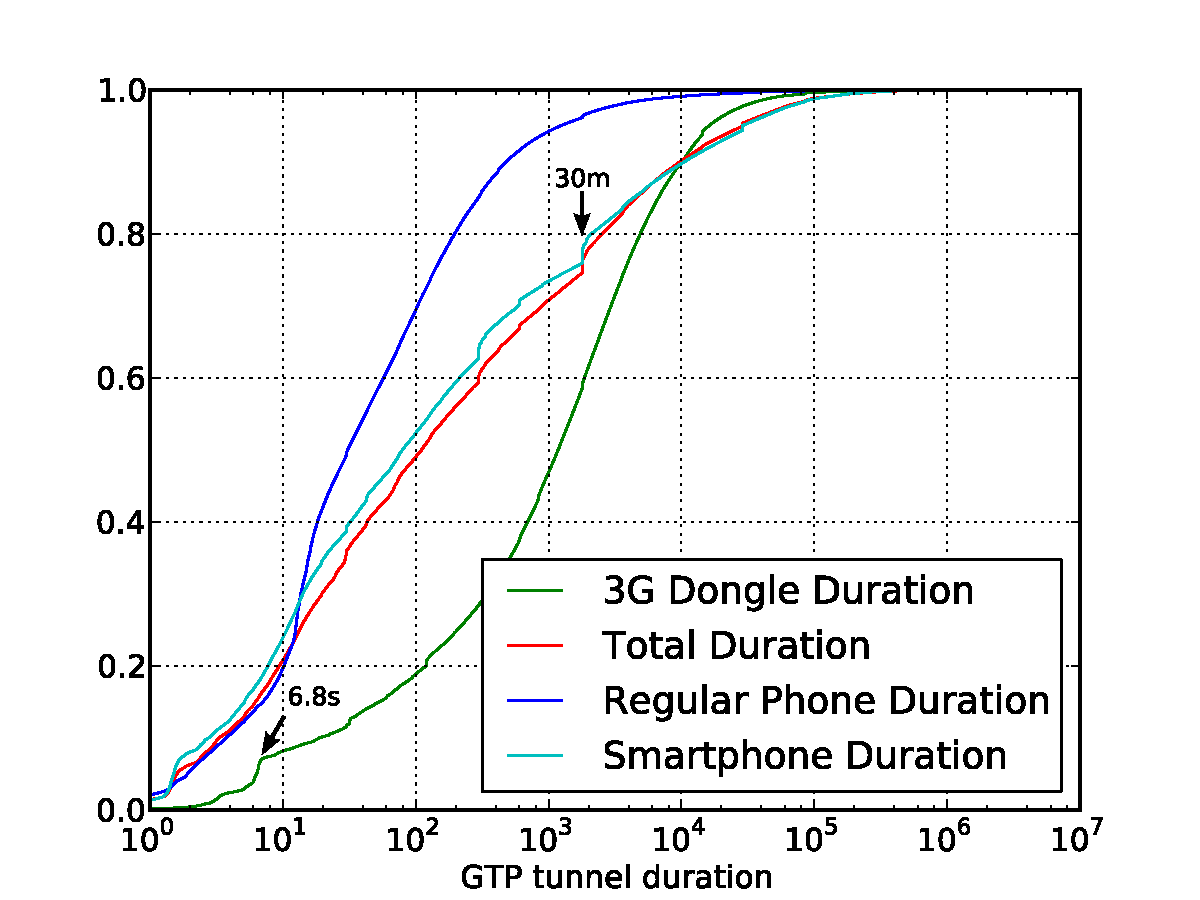
\includegraphics[width=\columnwidth]{images/tunnel-dur-class-cdf-mod.pdf}
    \caption{Tunnel duration distribution, separated for 3G dongles, smartphones and regular phones with medians at 115s (Total), 31s (Regular), 82s (Smartphone), and 1207s (3G Dongle)}
    \label{c4:fig:cdf-duration-device-class}
\end{figure}

Figure~\ref{c4:fig:cdf-duration-device-class} shows the empirical cumulative distribution functions for the PDP Context durations in our dataset. We distinguish the total duration distribution as well as the the distributions for smartphones, regular phones, and 3G dongles. It can be observed that tunnel durations range between mere seconds and more than one week\footnote{Although our dataset is just one week long, some tunnels started before the beginning of that week, and ended within it. Since the tunnel start dates were still available from the system, we chose to include the data.}.

The median is clearly different between device types, being much longer for 3G dongles than for mobile phones. This can probably be expected, as typical dongle sessions might involve working at a laptop for periods longer than a few seconds or minutes. Also, for the dongles, we observe less extremely long tunnels. Again, we could relate this to a hypothetical laptop working environment, where the device is used for a few hours but then shut down. With this, the PDP Context is deleted as well. 

Interestingly, the median duration of regular phones is higher than that of smartphones. This may indicate that smartphones regularly (and perhaps automatically) cause data traffic and therefore tunnels to occur. We conjecture this to be a first indication of the ``Angry Birds'' effect of automatically transferring small amounts of data, e.g. weather reports, stock exchange data, RSS feeds, or email notifications. We also observe two distinct steps, one at 6.8 seconds for dongles, and one at 30 minutes in the overall and smartphone distributions.


%%
\paragraph{Influence of the OS}
%%

\begin{figure}[htbp]
    \centering
    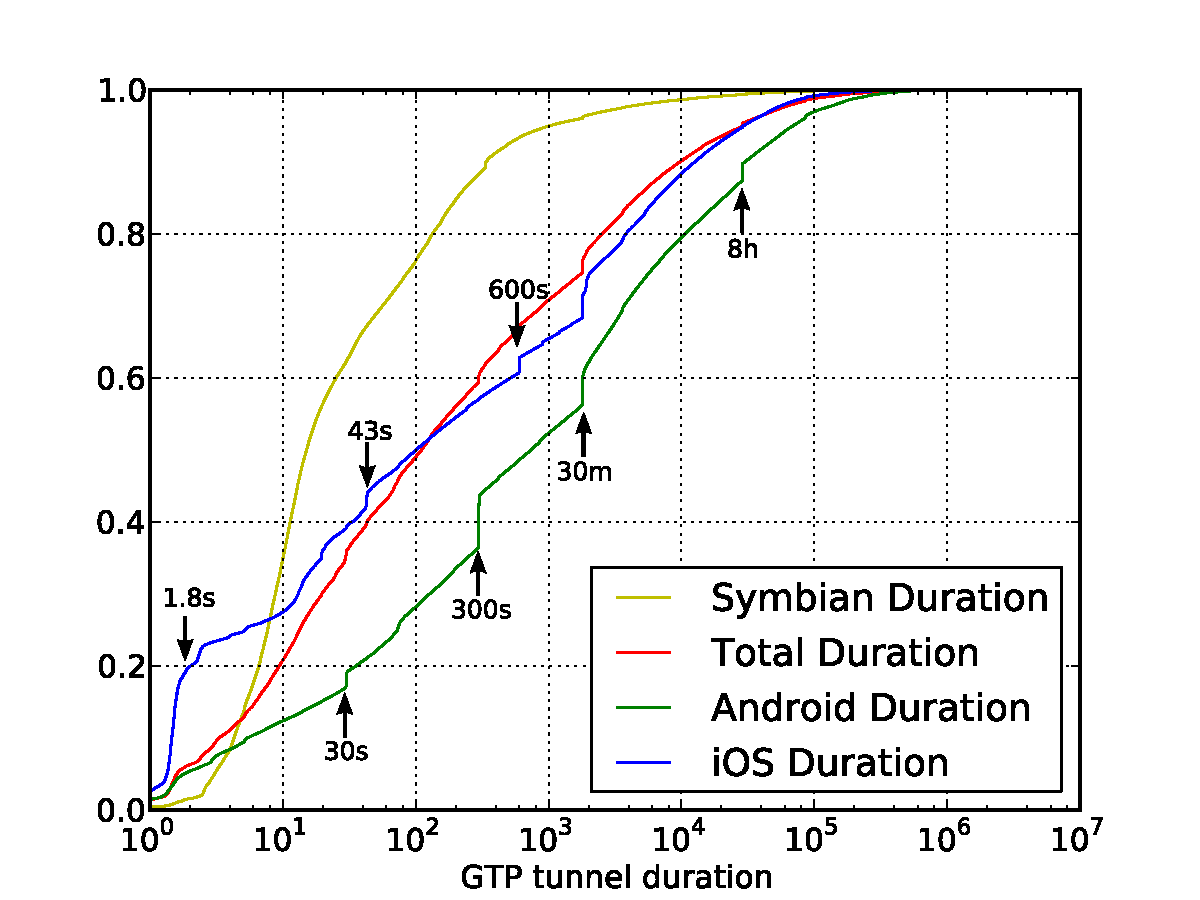
\includegraphics[width=\columnwidth]{images/tunnel-dur-os-cdf-mod.pdf}
    \caption{Tunnel duration cumulative distribution function, separated for Android and iOS devices; Medians at 115s (Total), 15.5s (Symbian), 104s (iOS), and 765s (Android)}
    \label{c4:fig:cdf-duration-os}
\end{figure}

Taking an even closer look at the smartphone device fraction, and differentiating the operating system to Symbian, Android, and iOS, we can still observe major differences as depicted in the empirical cumulative distribution functions of Figure~\ref{c4:fig:cdf-duration-os}. The tunnel duration distribution of the Symbian device fraction behaves much closer to the regular phones already depicted in Fig.~\ref{c4:fig:cdf-duration-device-class}. A possible explanation could be the user-base being more traditional, or the devices being feature phones whose behavior clearly differs from smartphones.

Again, a number of steps (i.e. accumulations of incidents) are visible in the distributions. Those that are only visible in one operating system type point to a source involving the device rather the network. This especially includes the 30 seconds, 300 seconds, and 600 seconds steps for Android, and the 600 seconds step for iOS devices. However, whether this behavior should be attributed to the operating systems themselves cannot be decided by only looking at these distribution. Other sources, e.g. the device's firmware version and user traffic dynamics need also be observed.

A last artifact of note are the large number of iOS devices with very short tunnel durations. Over 20\% of all tunnels established by these devices are shorter than two seconds. Our working hypothesis is, that this is an interaction between short regular traffic burst and a form of Fast Dormancy \cite{gsma2011fdbestpract} which iOS devices are known to implement, a technique to explicitly release radio resources. It is deemed to improve device battery life, radio signaling and radio spectrum efficiency. However, due to the earlier and more frequent radio state changes, it also could cause an increase in core network tunnel management signaling, which is probably what happened in the iOS case depicted in the CDF.



%%
\subsubsection{Impact of Categories on Total Signaling}
%%


\begin{figure}[htbp]
        \centering
        % \begin{subfigure}[b]{0.50\textwidth}
        %         \centering
        %         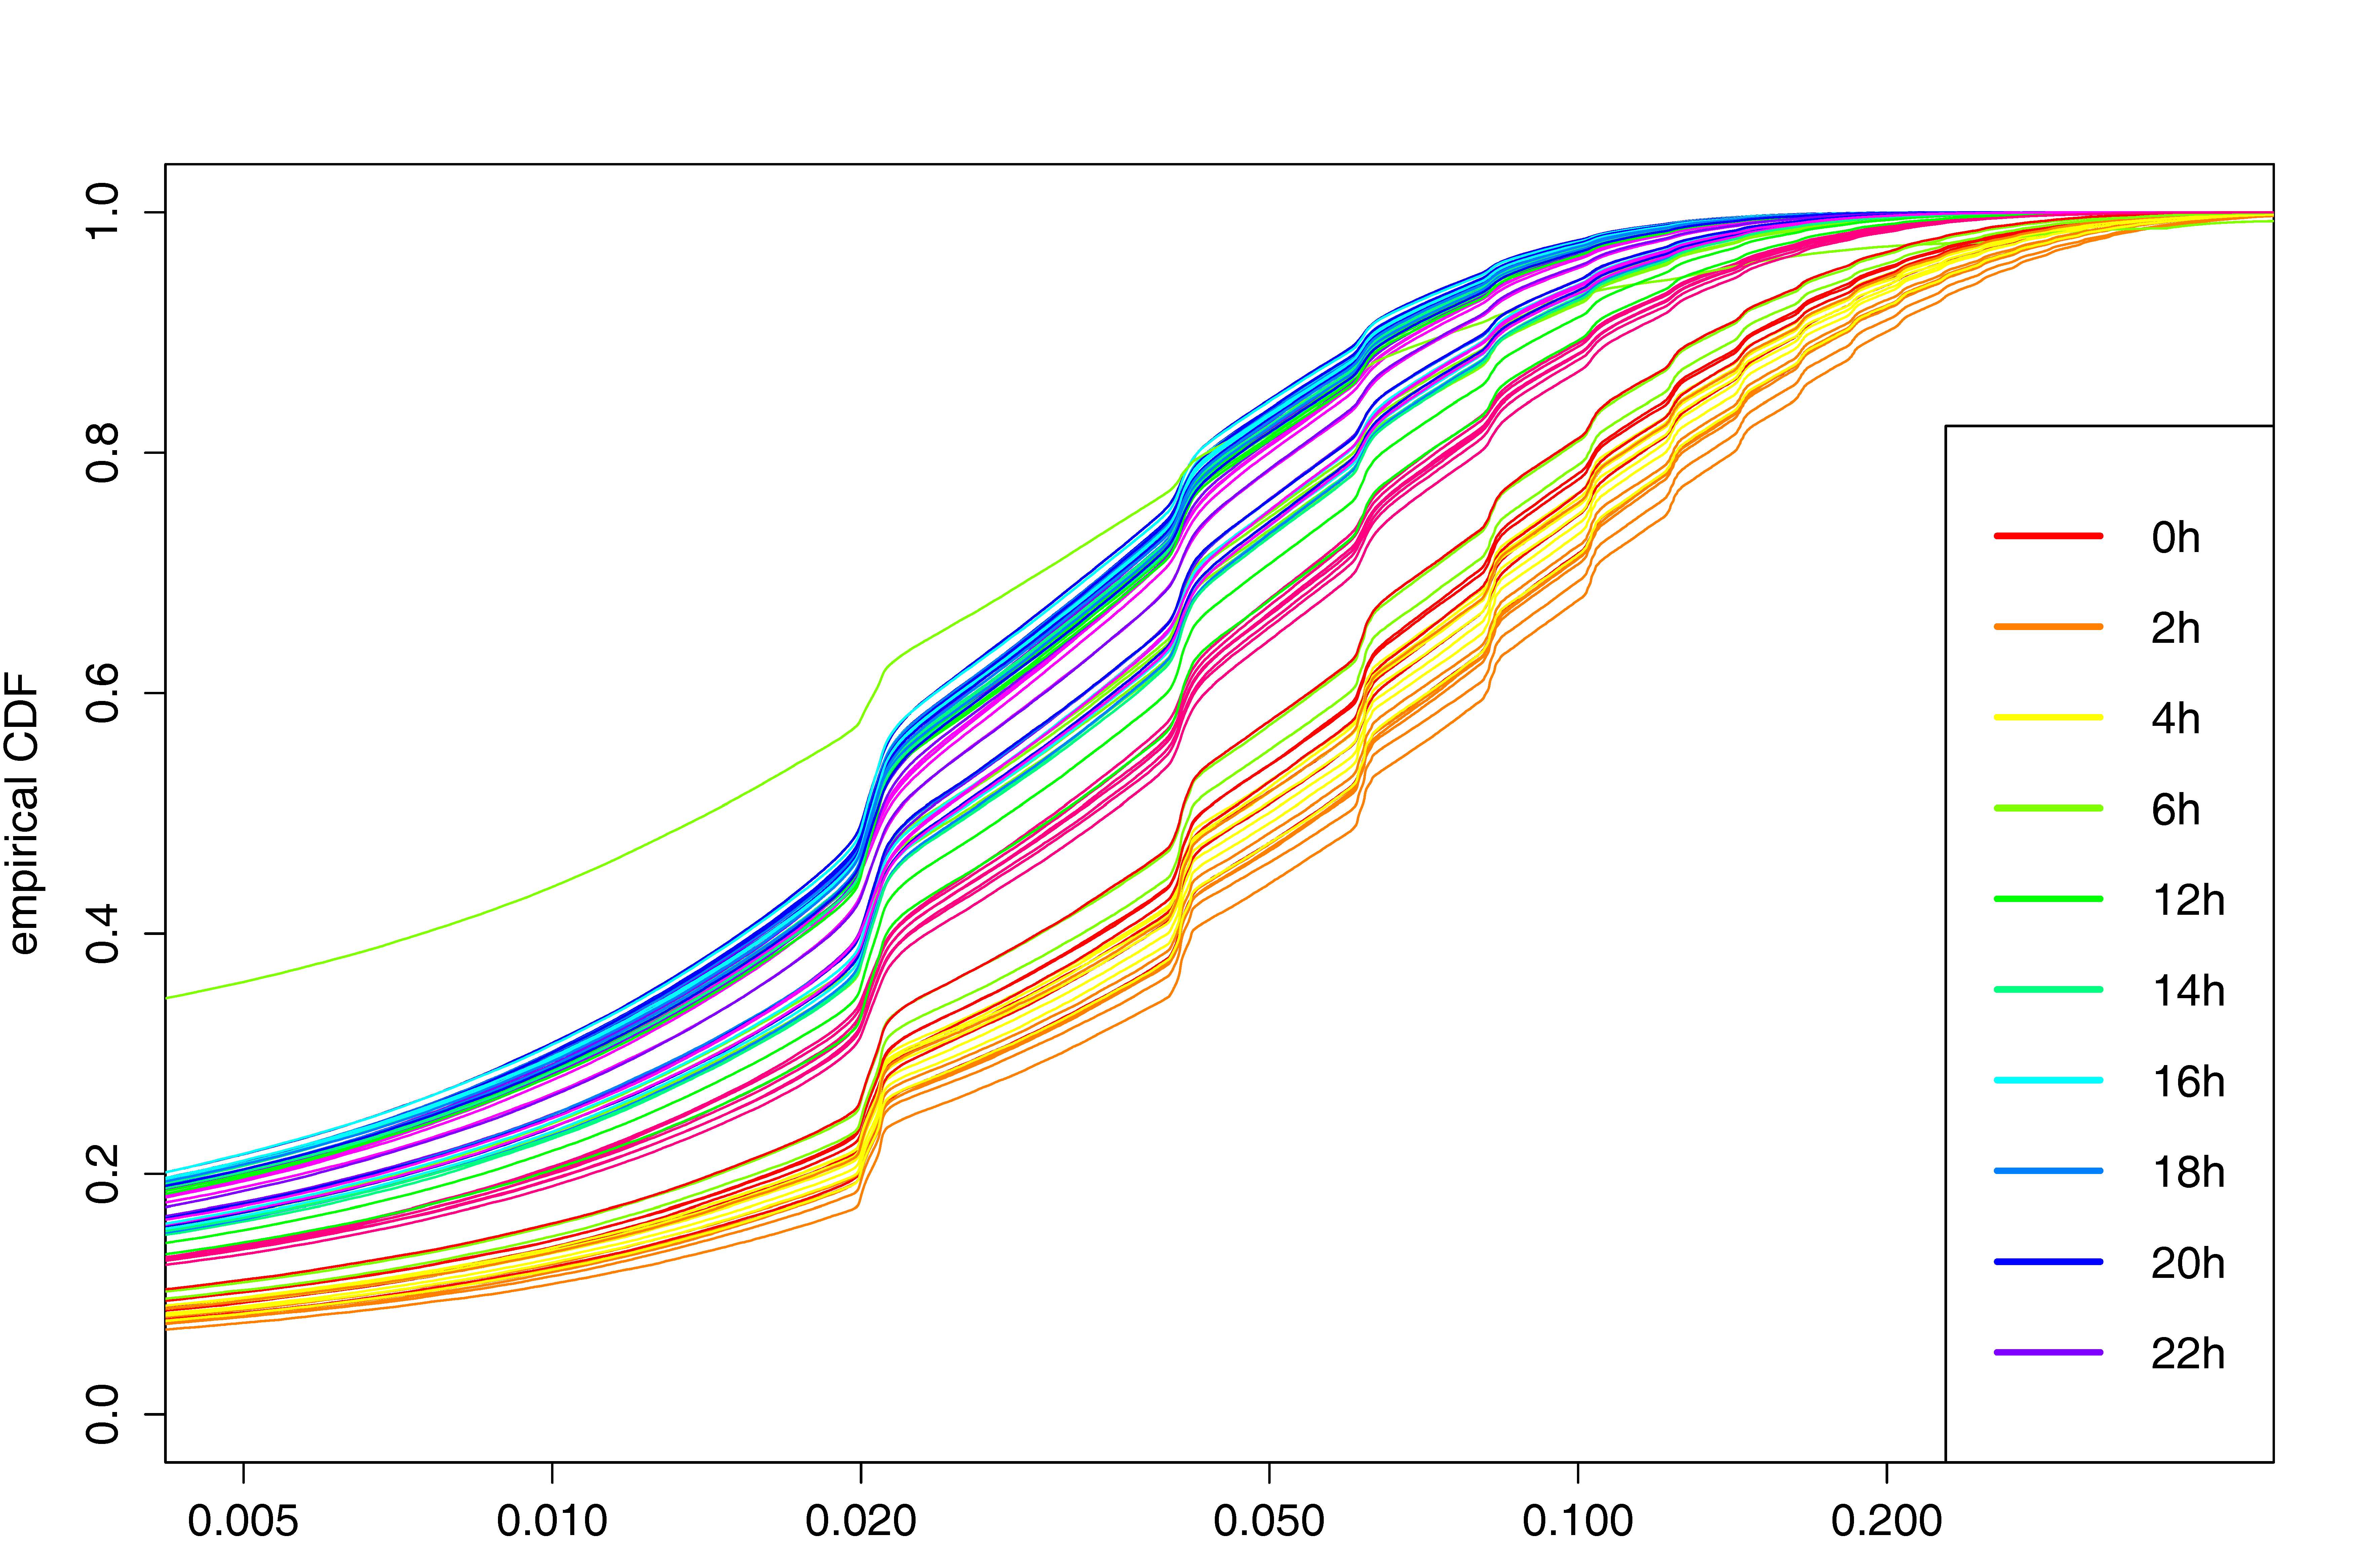
\includegraphics[width=\textwidth]{figures/R-IAT-ecdf-2h-log.png}
        %         \caption{All incoming tunnel requests.}
        %         \label{fig:IAT-ecdf-2h-all}
        % \end{subfigure}%
        %~ %add desired spacing between images, e. g. ~, \quad, \qquad etc.
          %(or a blank line to force the subfigure onto a new line)
        \begin{subfigure}[b]{0.50\textwidth}
            \centering
            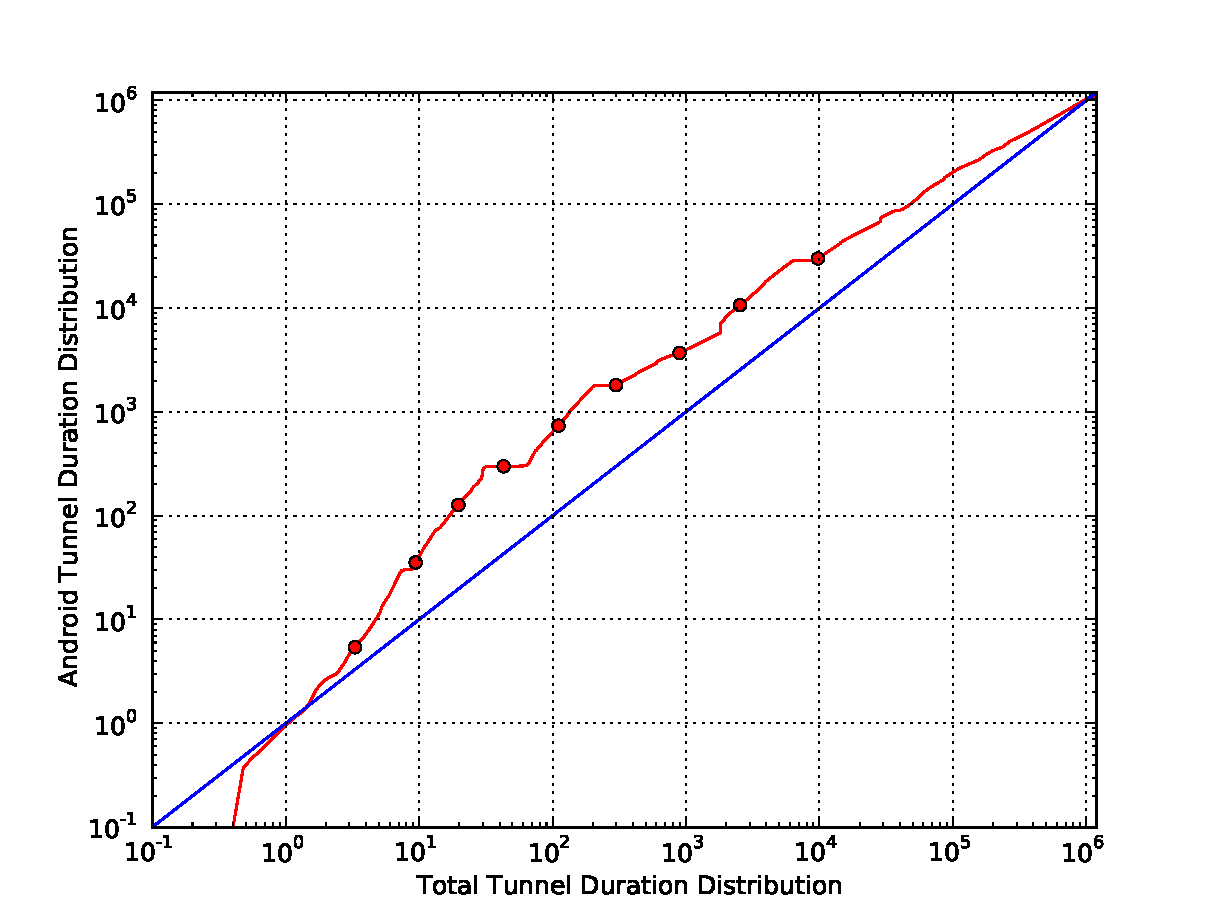
\includegraphics[width=\textwidth]{images/qq-total-vs-android.pdf}
            \caption{Android duration over the total duration.}
            \label{c4:fig:qq-total-vs-android}
        \end{subfigure}%
        ~
        \begin{subfigure}[b]{0.50\textwidth}
            \centering
            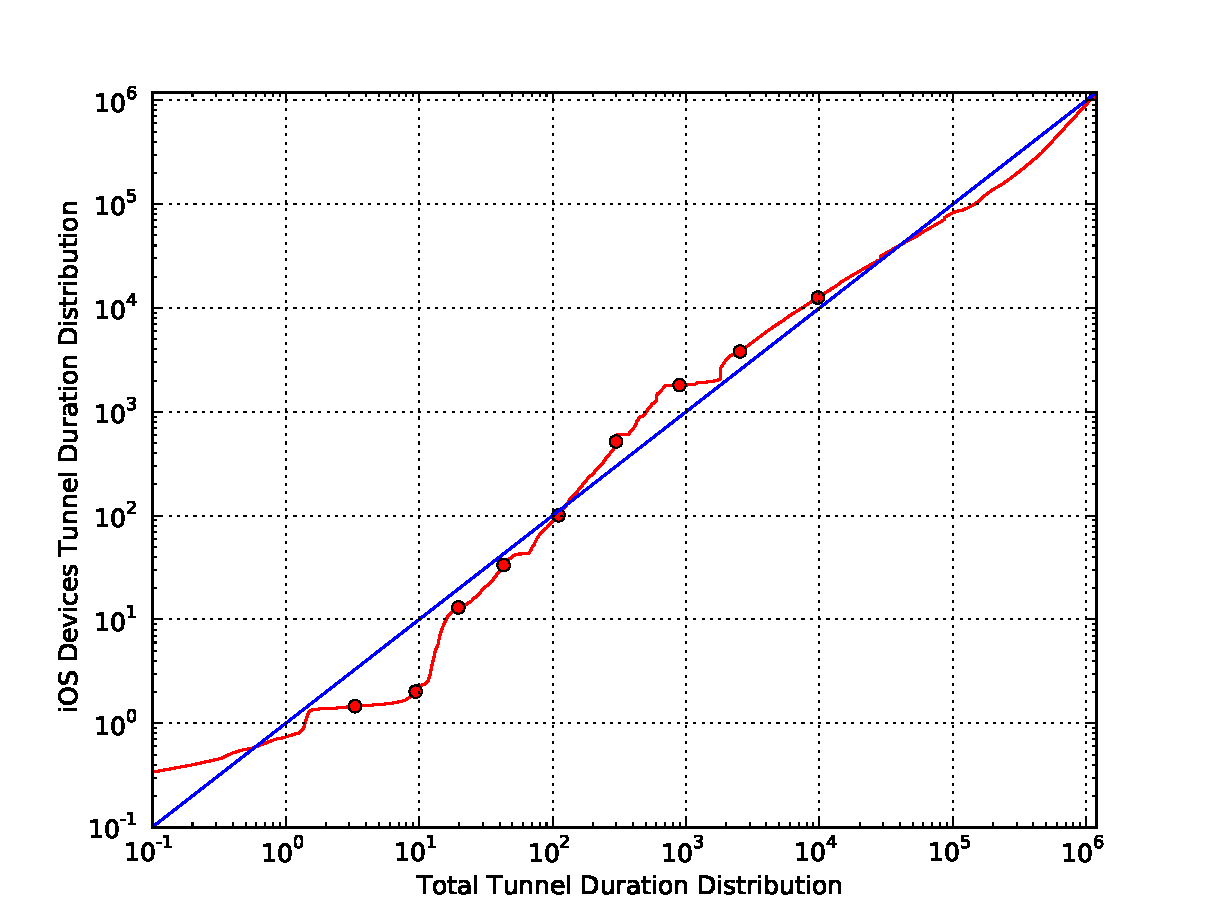
\includegraphics[width=\textwidth]{images/qq-total-vs-ios.pdf}
            \caption{iOS duration over the total duration.}
            \label{c4:fig:qq-total-vs-ios}
        \end{subfigure}

        \begin{subfigure}[b]{0.50\textwidth}
            \centering
            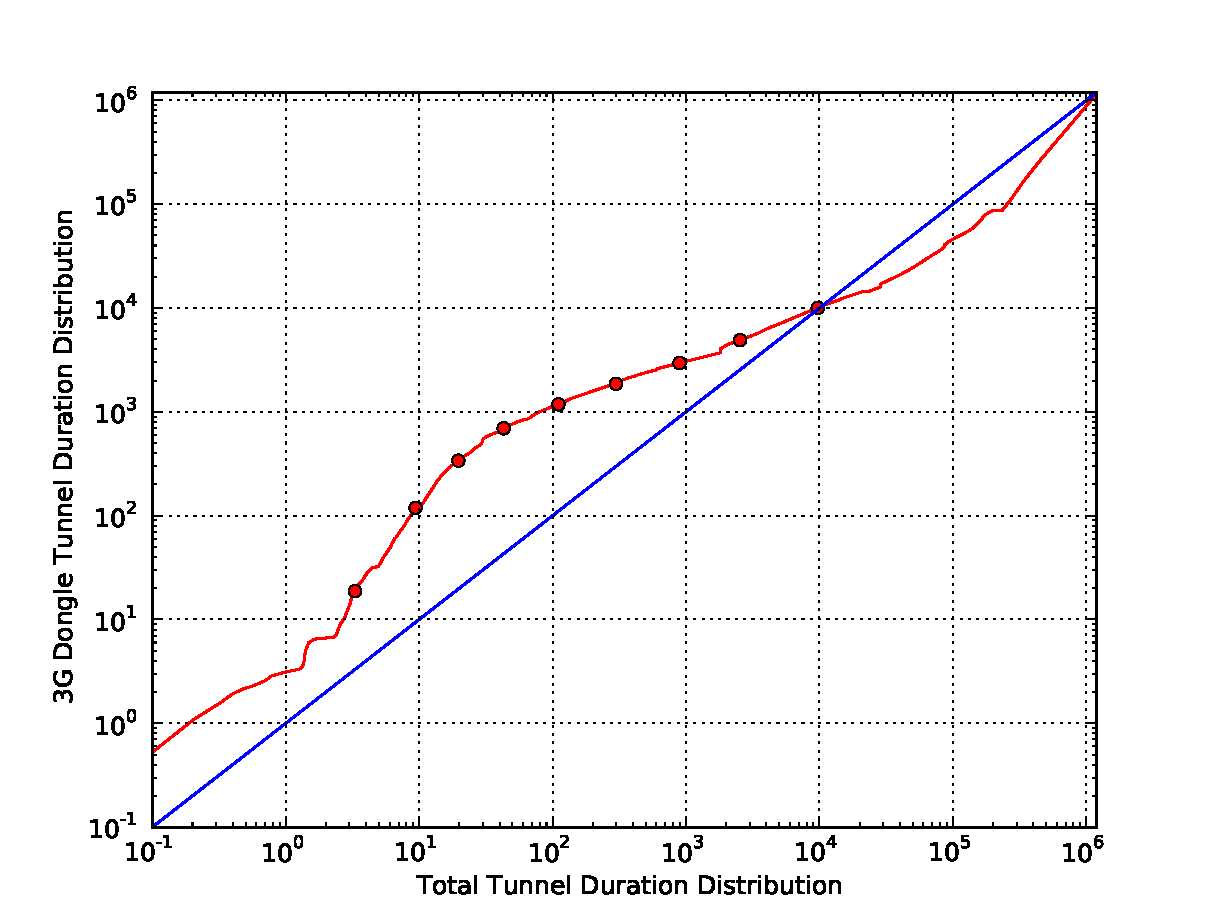
\includegraphics[width=\textwidth]{images/qq-total-vs-dongle.pdf}
            \caption{3G Dongle duratio over the total duration.}
            \label{c4:fig:qq-total-vs-dongle}
        \end{subfigure}%
        ~
        \begin{subfigure}[b]{0.50\textwidth}
            \centering
            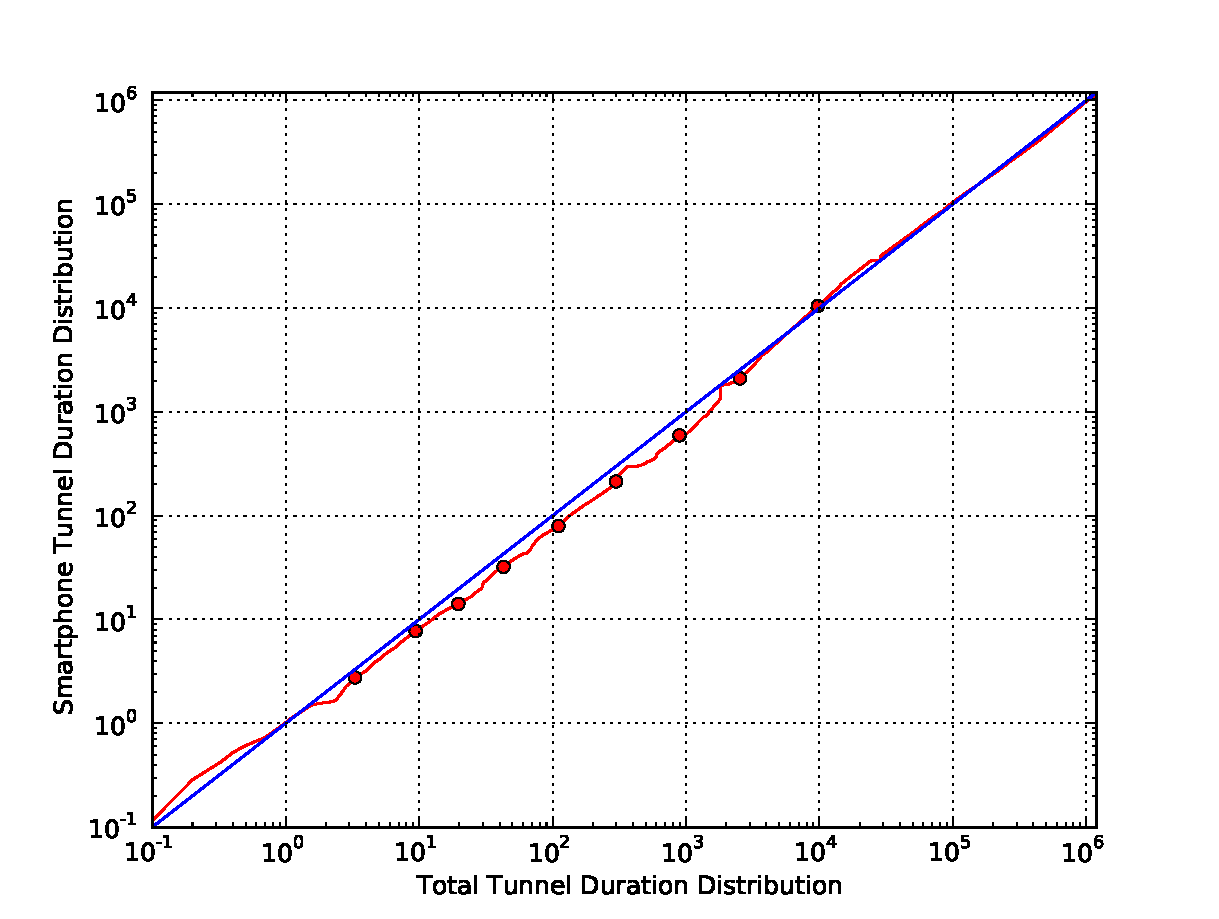
\includegraphics[width=\textwidth]{images/qq-total-vs-smartphone.pdf}
            \caption{Smartphone duration over the total duration.}
            \label{c4:fig:qq-total-vs-smartphones}
        \end{subfigure}
 \caption{Q-Q Plots of the tunnel duration distributions per operating system, with encircled deciles.}
\label{c4:fig:qq-plots}
\end{figure}



In an attempt to show which of the presented categories have an impact on the total duration (if at all), we present Q-Q plots of the various categorized durations against the total duration in Figure~\ref{c4:fig:qq-plots}. In theory, if both durations follow the same distribution, one expects a straight line through the origin at an angle of 45$^o$. A steeper incline indicates less densely spaced values in the distribution at the y axis. Looking at igures~\ref{c4:fig:qq-total-vs-android} and \ref{c4:fig:qq-total-vs-ios} which compare different operating systems, both similar and dispersing parts can be observed. While tunnel durations on Android  are more similarly distributed for the shorter and longer durations, iOS device tunnel durations are most similar to the overall tunnel duration distribution in the middle range of values.

Combining all types of smartphones together and comparing them to the other major player in any mobile network, the 3G dongles, we observe in Figure \ref{c4:fig:qq-total-vs-smartphones} that both the total and the smartphone durations are almost equally distributed (except for minor variations). On the other hand, 3G dongles follow a very different distribution, see Figure \ref{c4:fig:qq-total-vs-dongle}. Their effect on tunnel management signaling seems to be negligible despite the  large amount of traffic they are causing. Therefore, we conclude that planning and dimensioning of the control plane needs to keep smartphone behaviors more closely in mind than that of other device types.


\begin{figure}[htbp]
	\centering
	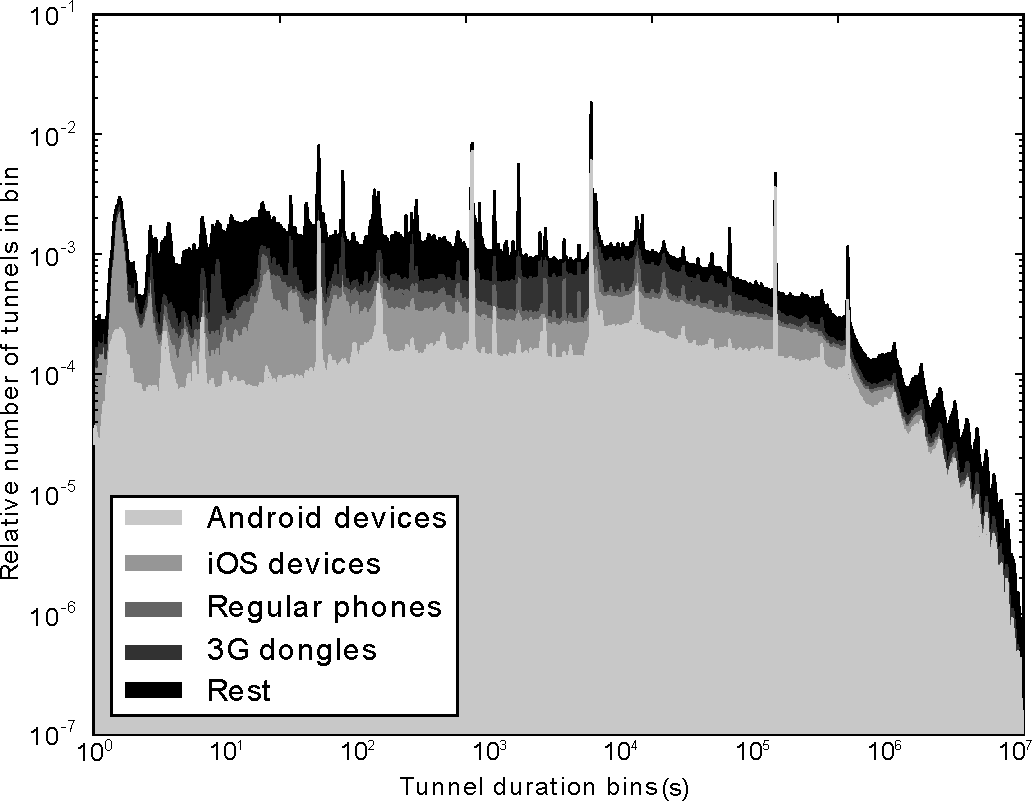
\includegraphics[width=1.0\textwidth]{images/stacked-durations-2-fixed.pdf}
	\caption{Stacked logscale bin plot of the number of tunnels with duration in this bin; classified by Android, iOS and 3G dongles.}
	\label{c4:fig:stacked-durations}
\end{figure}

Figure~\ref{c4:fig:stacked-durations} shows another interesting influence the operating system has on signaling in the mobile core network. This plot shows the relative number of tunnels with a duration in one of 1000 logarithmically scaled bins, stacked by OS category on top of each other. As with the separate distributions, we discover that the durations are not evenly distributed, but rather follow sharp spikes. The largest spike across all categories is the one at a duration of 30 minutes, making up about 1.8\% of all tunnels in the network. Since this spike happens across all device types, we think this makes a rather strong case for being network-induced, and an indication for the aforementioned possible IDLE state transition. On the other hand, the bulk in the short-to-medium ranges of tunnel duration is rather not governed by the two major smartphone operation systems but by other devices in the network, which do not show major spikes in other bins. We can also recognize a long-tail behavior in the distribution of tunnel durations.

%iOS: over 20\% of tunnels shorter than two seconds. 

%\begin{table*}
%\centering
%\caption{Relative \acs{TAC} Statistics.}
%\label{tab:tacstats}
%\begin{tabular}{|p{4cm}|p{2cm}|p{2cm}|p{2cm}|p{2cm}|p{2cm}|} \hline
%& \textbf{\# of Flows} & \textbf{Ratio of Traffic} & \textbf{\# of Tunnels} & \textbf{\# of GTP Signalling Msgs} & \textbf{\# of Distinct \acp{MS-ID}}%\\ \hline
%Total 			& 2234659247 	& 122758578593993	& 16632094 	& 409733865	& 1255293 (from GTPdb) / 1030895 (from flow db) \\ \hline
%Have entry in TAC DB 	& 99.72\% 	& 99.97\%	& 87.57\% 	& 90.95\% 	& 80.93\% \\ \hline
%Classified as smartphone& 20.58\% 	& 12.81\%	& 60.31\% 	& 75.99\% 	& 37.97\% \\ \hline

%as regular phone 	& 0.26\% 	& 0.37\%	& 5.40\% 	& 0.94\% 	& 9.25\% \\ \hline
%as 3G dongle		& 66.55\% 	& 75.12\%	& 12.71\% 	& 9.53\% 	& 25.10\% \\ \hline
%Running on Android	& 10.82\% 	& 6.48\%	& 14.33\% 	& 43.33\% 	& 14.01\% \\ \hline
%iOS			& 7.22\% 	& 4.47\%	& 18.91\% 	& 20.35\% 	& 7.94\% \\ \hline
%S40 / S60 / Symbian	& 1.02\% 	& 1.09\%	& 21.17\% 	& 4.51\% 	& 12.97\% \\ \hline
%Blackberry OS		& 0.07\% 	& 0.10\%	& 2.17\% 	& 2.60\% 	& 1.48\% \\ \hline
%\end{tabular}
%\end{table*}



%%
% Influence of the Radio Access Type
%%
%TODO: radio access type plots, if we have the data
%
%\begin{figure}
%\centering
%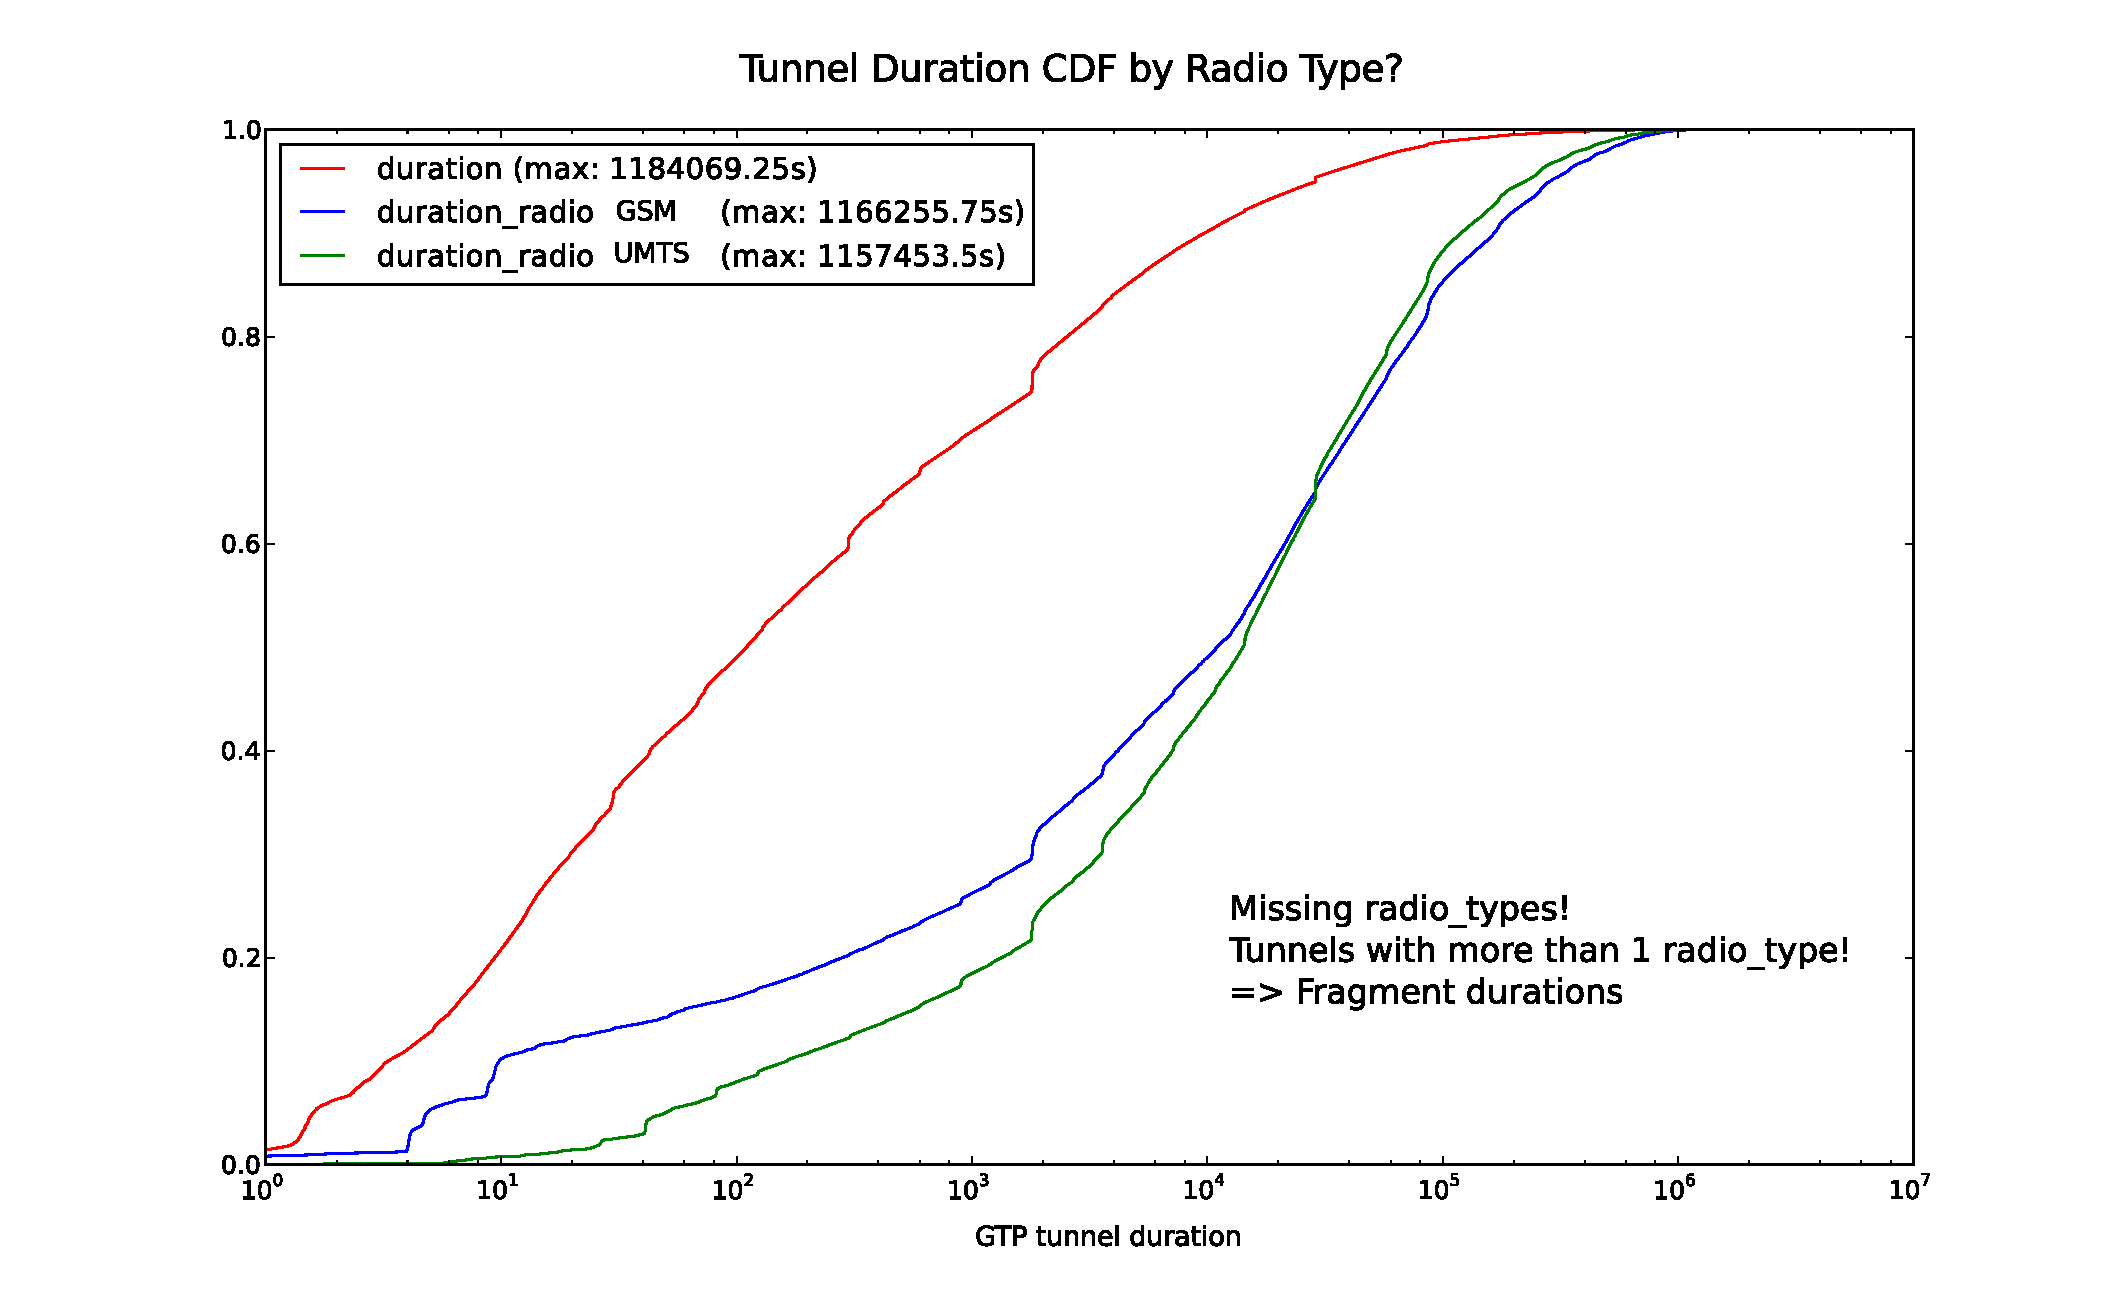
\includegraphics[width=\columnwidth]{figures/tunnel-dur-radio-cdf-mod.pdf}
%\caption{Tunnel duration distribution, separated for UMTS and GPRS radio access [NOTE: only in the last tunnel segment; and majority of radio types %is unknown anyway.}
%\label{fig:cdf-duration-radio}
%\end{figure}

% 10/30m jumps can be seen on android, but not on iOS, why?
%  maybe fast dormancy?

%Corner Cases: 
% - Tunnels active longer than the measurement duration, i.e. either CREATE or DELETE message outside of the one week time span


%We search for factors influencing tunnel durations, and discuss if and how we can observe them in the data set. Thereafter we build up our proposed classification based on these factors.

% User behavior factors, mobility
% Factors from the device: OS, firmware
% Network side factors
% Protocol factors: RRC state change, timeouts

% typical CELL\_PCH to IDLE transition timer 10 to 30 mins
% does/can this influence core sgsn<->ggsn tunnels?
% when is a tunnel deleted?
% data can still flow when in CELL\_PCH, so probably only in IDLE?
% give references to specs!

%On of our goal in our evaluation was to distinguish between certain device types and classes. 

%\begin{table}
%\centering
%\caption{TAC Statistics}
%
%\begin{tabular}{|p{2cm}|p{2cm}|p{2cm}|p{2cm}|} \hline
%& \textbf{\# of Flows} & Total Traffic (Bytes) & Upstream (Bytes) & Downstream (Bytes) & \textbf{\# of Tunnels} & \textbf{\# of GTP Signalling Msgs} & \textbf{\# of Distinct IMSIs}\\ \hline
%Total 			& 2234659247 	& 122758578593993 (112TB) 	&  &  	& 16632094 	& 409733865	& 1255293 (from GTPdb) / 1030895 (from flow db) \\ \hline
%Available in TAC DB 	& 2228315260 	& 122716712007150 (111.61TB) 	&  &  			& 14565430 	& 372662108	& 1015891 \\ \hline
%Classified as smartphone& 459990512 	& 15721818747754 (14.30TB)	&  &  			& 10030734 	& 311342846 	& 476675 \\ \hline
%as regular phone 	& 5705832 	& 448140315058 (0.41TB)		&  & 			& 897529 	& 3860162	& 116124 \\ \hline
%as 3G dongle		& 1487230062 	& 92215931895630 (83.87TB) 	&  & 			& 2114756 	& 39053819 	& 315003 \\ \hline
%Running on Android	& 241973565 	& 7953178401958	(7.2TB)		&  & 			& 2383255 	& 177537567 	& 175919\\ \hline
%iOS			& 161408903 	& 5481693567152 (5TB)		&  & 	& 3145384 	& 83374590 	& 99679 \\ \hline
%S40 / S60 / Symbian	& 22827418 	& 1332996529271 (1.21TB) 	&  & 			& 3520242 	& 18479002 	& 162790 \\ \hline
% blackberry 128074907884 (0.12TB)
%\end{tabular}
%\end{table}

%Devices with GTP signaling but no user plane traffic: (\#distinct imsis gtp db)-(\#distinct imsis flow db):

% $255293-1030895=224398\text{ or }17.88\%$


%different tacs for same devices with >1M units as the unit identifier part of the IMEI would otherwise overflow 



% One week in April 2011 (04/11/2011 up to including 04/17/2011) measured at one SGSN-GGSN path, about half of the total traffic of the operator.
%Containing user traffic flow aggregated data; Entry for every GTP control plane message on the path, including success/failure status codes





%%%%%%%%%%%%%%%%%%%%%%%%%%%%%%%%%%%%%%%%%%%%%%%%%%%%%%%%%%%%%%%%%%%%%%%%%%%%%%%
\subsection{Core Network Load Statistics}

Having characterized the dataset available to us we now shed some light on the control plane and load dynamics in a mobile core network and attempt to show the possible impact of certain devices or other properties of the network. 




%%%%%%%%%%%%%%%%%%%%%%%%%%%%%%%%%%%%%%%%%%%%%%%%%%%%%%%%%%%%%%%%%%%%%%%%%%%%%%%
\subsection{Individual Examinations}

To examine some of these factors, we present the following number of individual investigations. Our measure of choice are the GTP tunnels as they carry lots of meaning in being directly related to the signaling amount in the network. We investigate their duration as well as the number of arrivals and look at a measure for the processing time of events at the GGSN. These insights will also allow us to build a simple toy model for the core network load in the next chapter.





%%%%%%%%%%%%%%%%%%%%%%%%%%%%%%%%%%%%%%%%%%%%%%%%%%%%%%%%%%%%%%%%%%%%%%%%%%%%%%%
\subsubsection{Tunnel Number of Arrivals and Inter-Arrival Time}

While tunnel durations and the involved signaling at the beginning and end of the duration is one aspect of control plane load, the number of tunnel arrivals might be another, which we are looking into in this section.

In addition to describing the arrival process on the basis of the number of arrivals, we also take a look at the tunnel inter-arrival time. Specifically, with this process we mean the arrival of tunnel requests, i.e. GTP CREATE requests, at the \gls{GGSN}. This also adds to the foundation of the load model constructed in the next chapter. 

\begin{figure}[htbp]
	\centering
	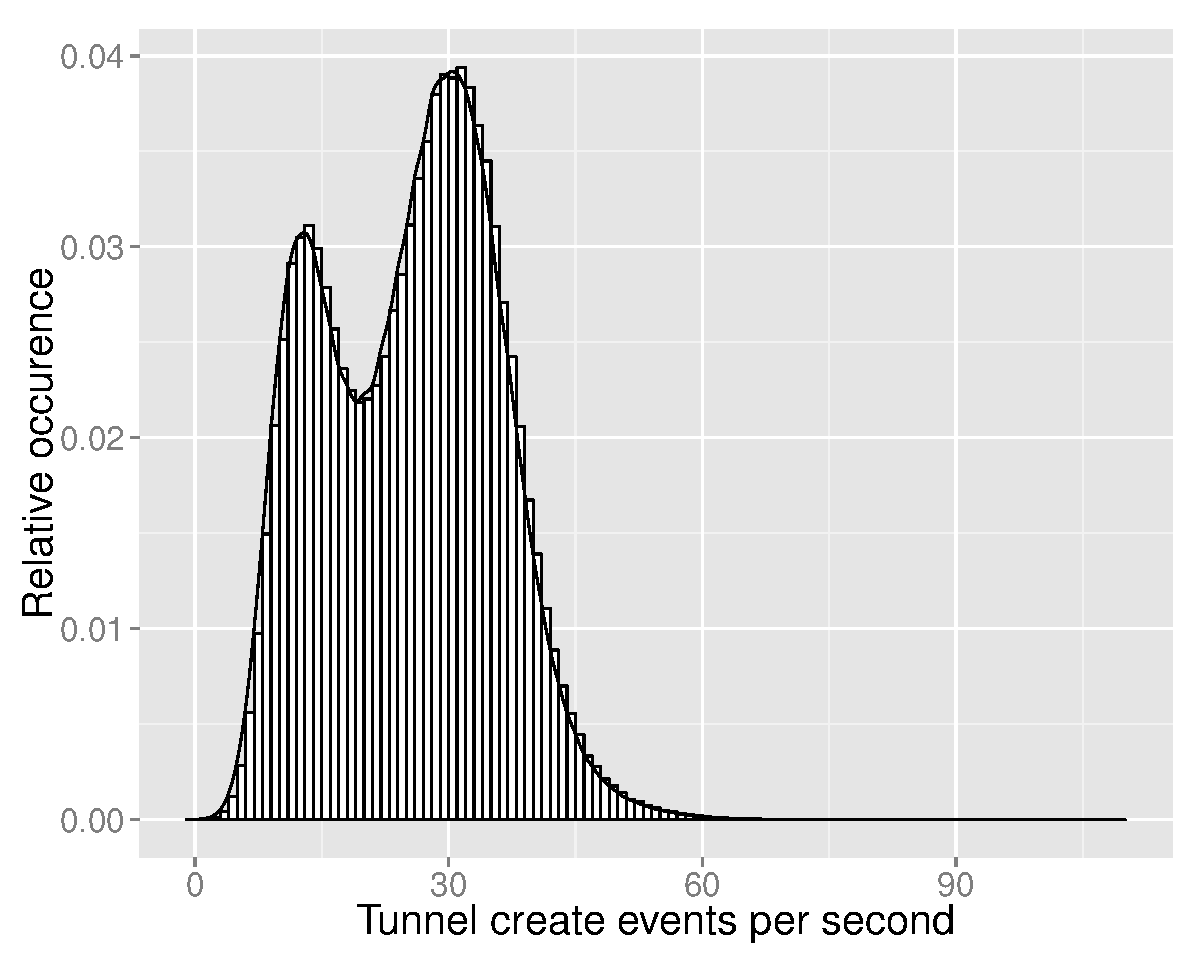
\includegraphics[width=\columnwidth]{images/create_freq.pdf}
	\caption{Tunnel arrivals in one second intervals.}
	\label{c4:fig:freq-arrivals}
\end{figure}

Figure \ref{c4:fig:freq-arrivals} depicts the number of arrivals per second during the whole weeklong period. Of note is the clear bimodal nature with one peak around twelve and the other in the low thirties. While the distribution is rather compact around these two peaks, there are some clear outliers up to 107.
If we again hypothesize that an increased number of arrivals means higher load in the network, we can assume that load is not constant but rather switches between two modes with some periods with extraordinary load induced by an increased number of arrivals.

\begin{figure}[htbp]
	\centering
	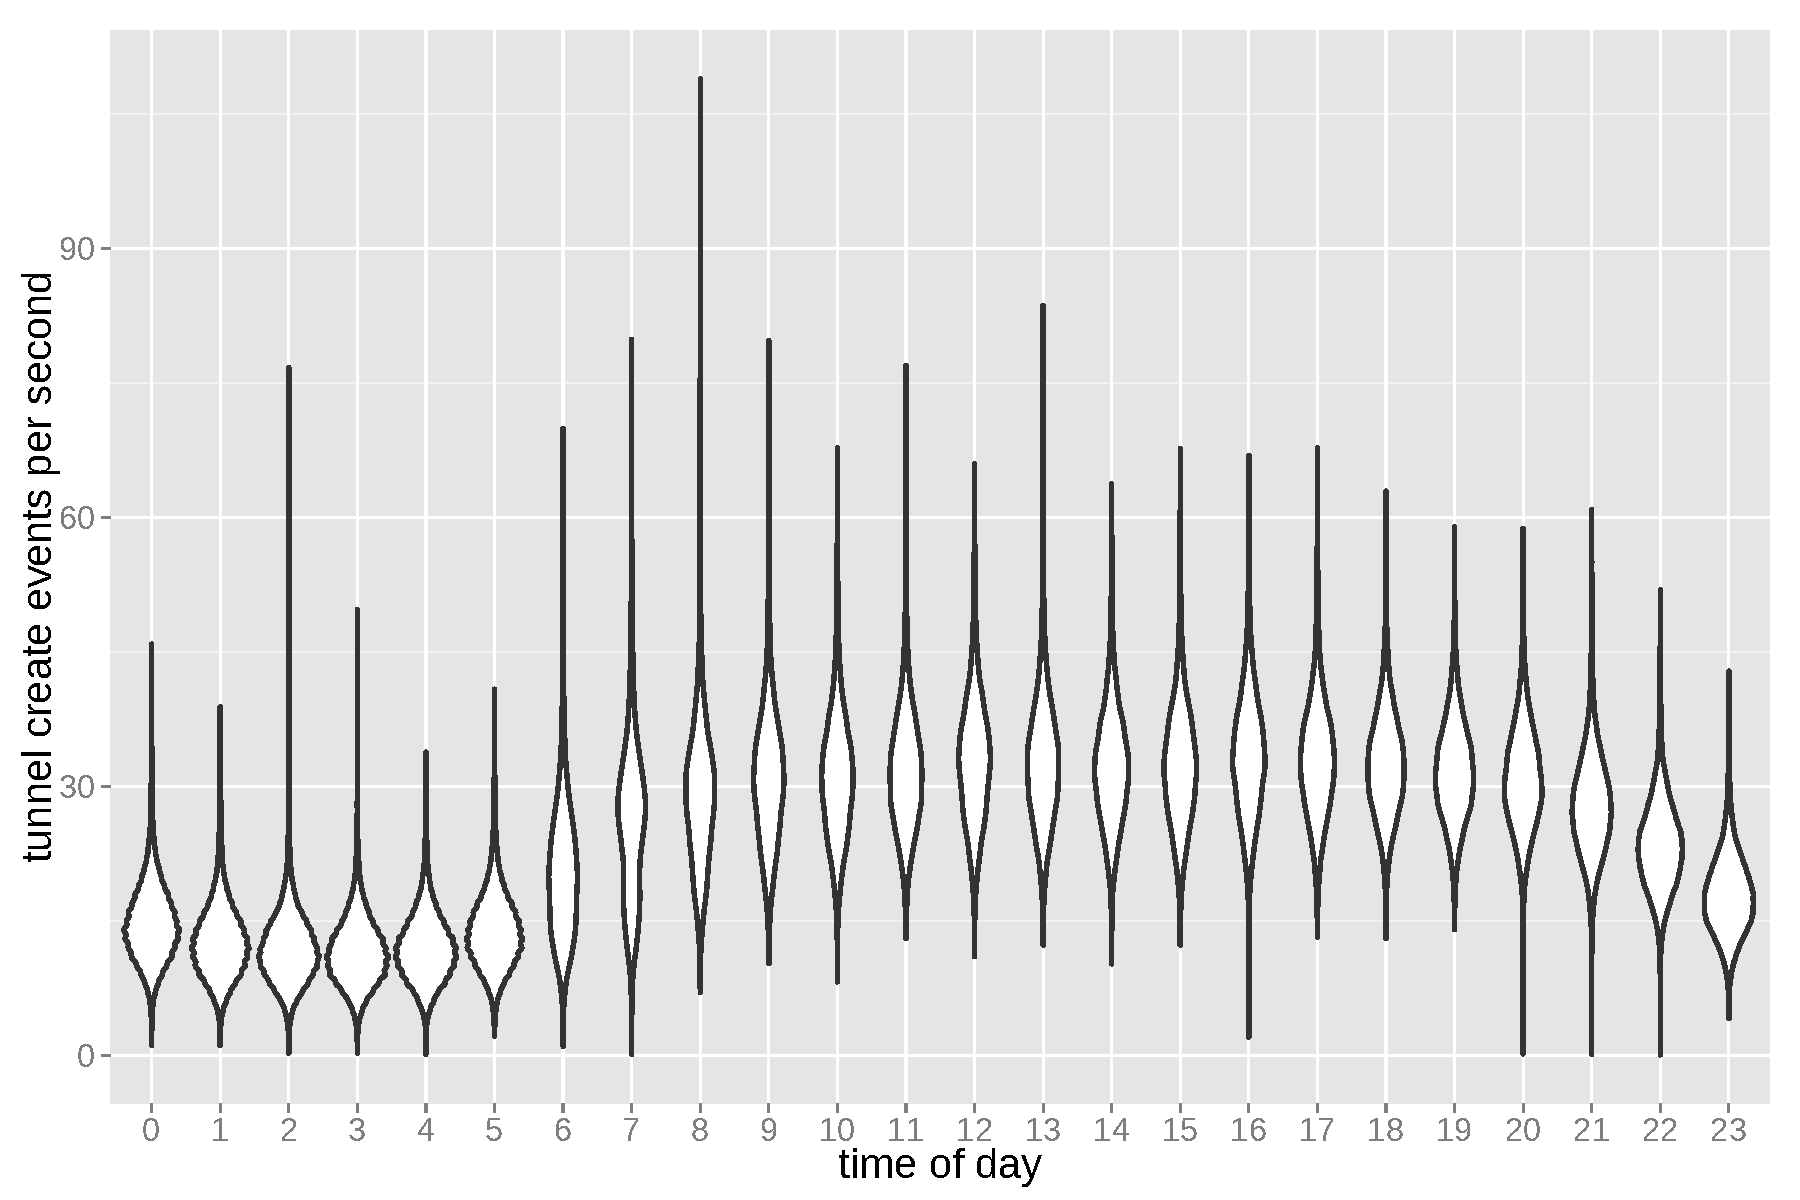
\includegraphics[width=\columnwidth]{images/R-createspersecond-1h-violin.pdf}
	\caption{Violin plot of tunnel arrivals in one second per time of day.}
	\label{c4:fig:freq-arrivals-per-second-violin}
\end{figure}

To find the cause of these two modes we take a peek at the diurnal arrival pattern. Figure \ref{c4:fig:freq-arrivals-per-second-violin} contains a violin plot showing again the arrivals per second but broken down by time of day. A violion plot, while being similar to a box plot, additionally shows the density of the individual items on the vertical axis.
The nocturnal median from around midnight to 5am and the longer daytime median, 8am to 19pm, closely resemble the two modes found in the histogram. In between are short transition phases. Notably, during daytime the arrivals and their densities are spread out on a much larger value range. This could be an indication of load fluctuations in the system.


\begin{figure}[htbp]
        \centering
\makebox[\textwidth]{        
        \begin{subfigure}[b]{0.45\paperwidth}    
                \centering
                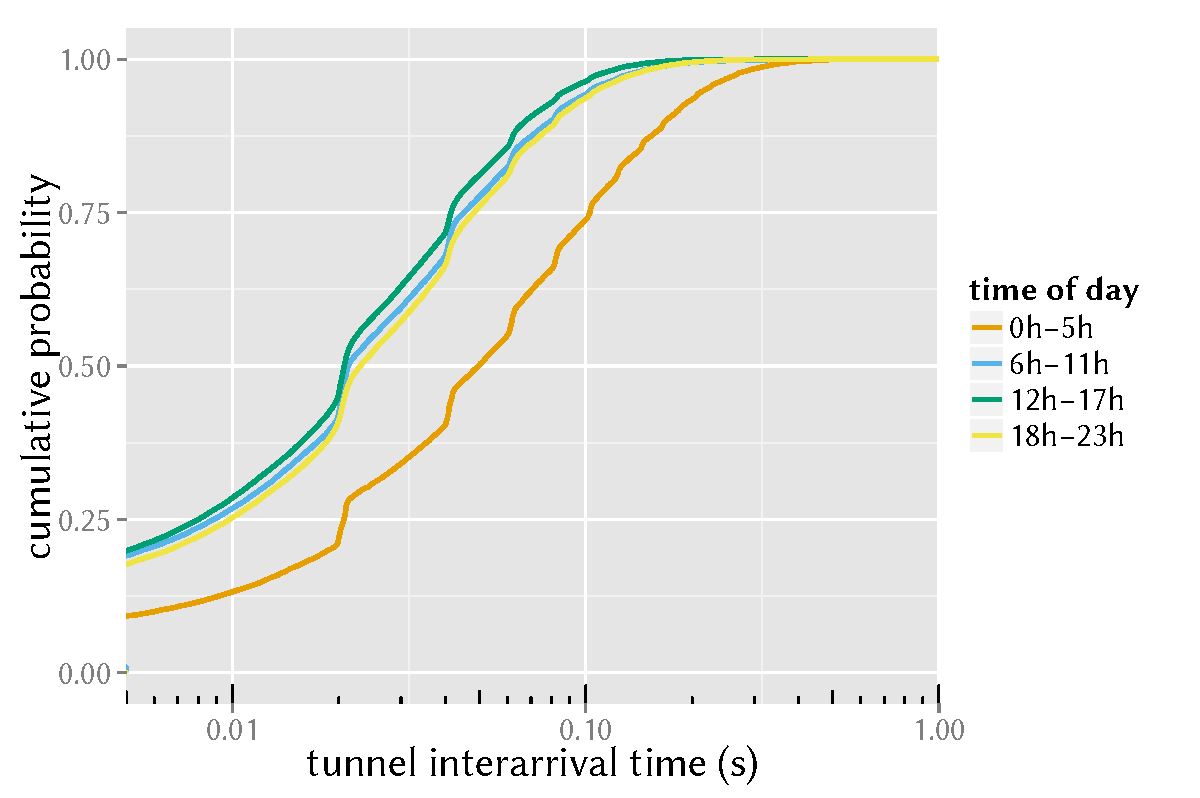
\includegraphics[width=\textwidth]{images/R-IAT-all-2h-ecdfs.pdf}
                \caption{All tunnel requests.}
                \label{c4:fig:IAT-ecdf-2h-all}
        \end{subfigure}%
        ~
        \begin{subfigure}[b]{0.45\paperwidth}
                \centering
                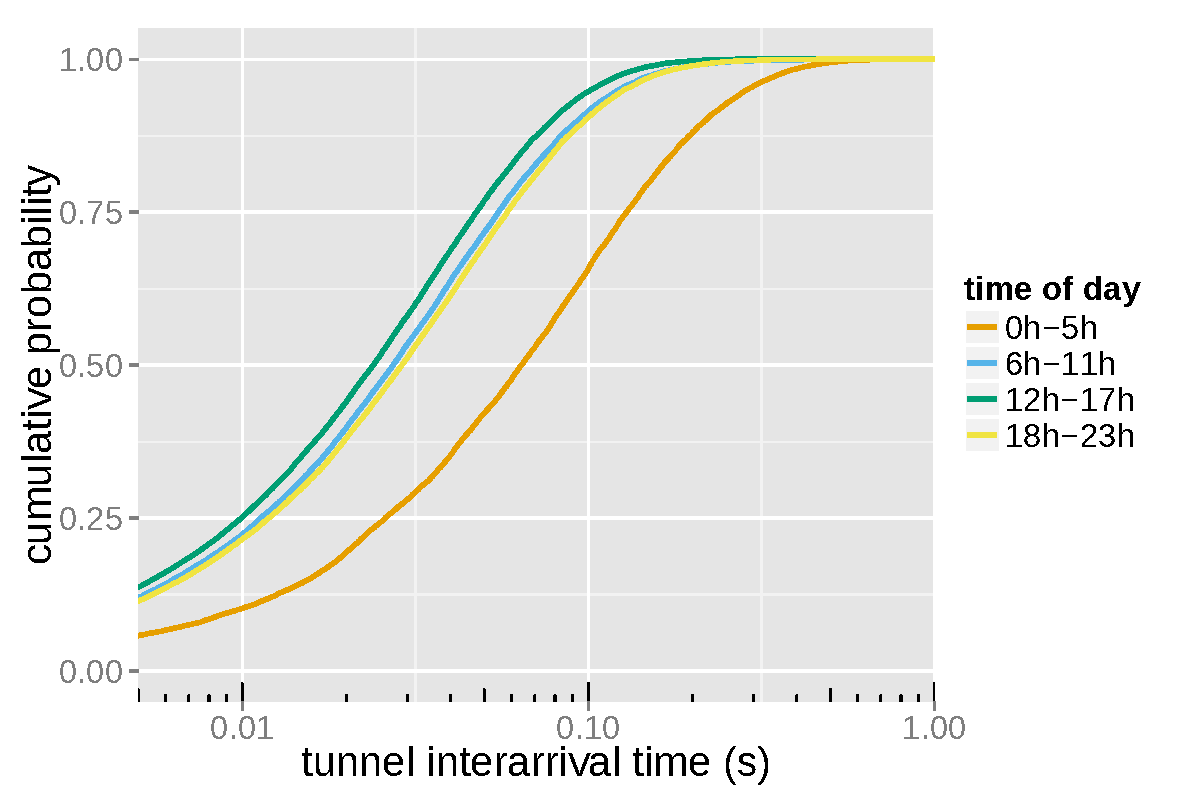
\includegraphics[width=\textwidth]{images/R-IAT-fromflows-ecdfs-2h.pdf}
                \caption{Only tunnels with data flows.}
                \label{c4:fig:IAT-ecdf-2h-active}
        \end{subfigure}
        }

 \makebox[\textwidth]{    
        \begin{subfigure}[b]{0.45\paperwidth}
                \centering
                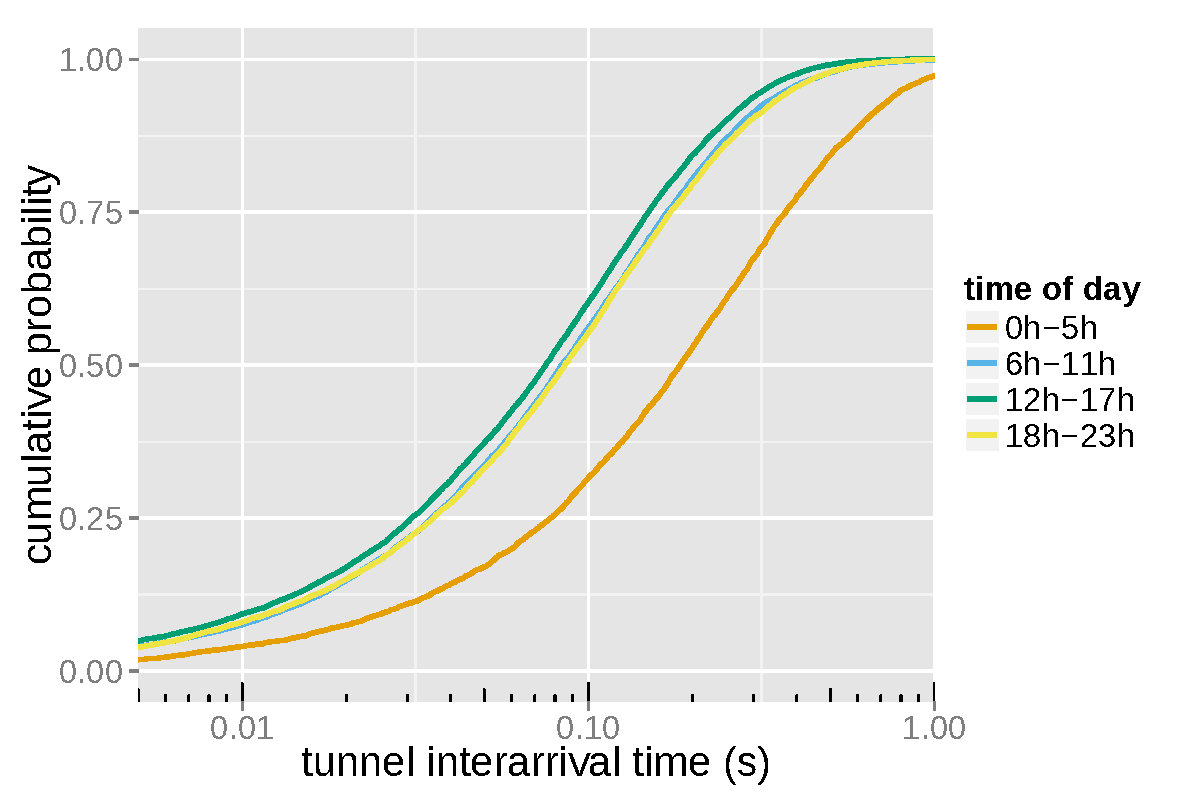
\includegraphics[width=\textwidth]{images/R-IAT-fromflows-gprs-ecdfs-2h.pdf}
                \caption{Tunnels with data flows initiated in GPRS.}
                \label{c4:fig:IAT-ecdf-2h-active-gprs}
        \end{subfigure}%
        ~
        \begin{subfigure}[b]{0.45\paperwidth}
                \centering
                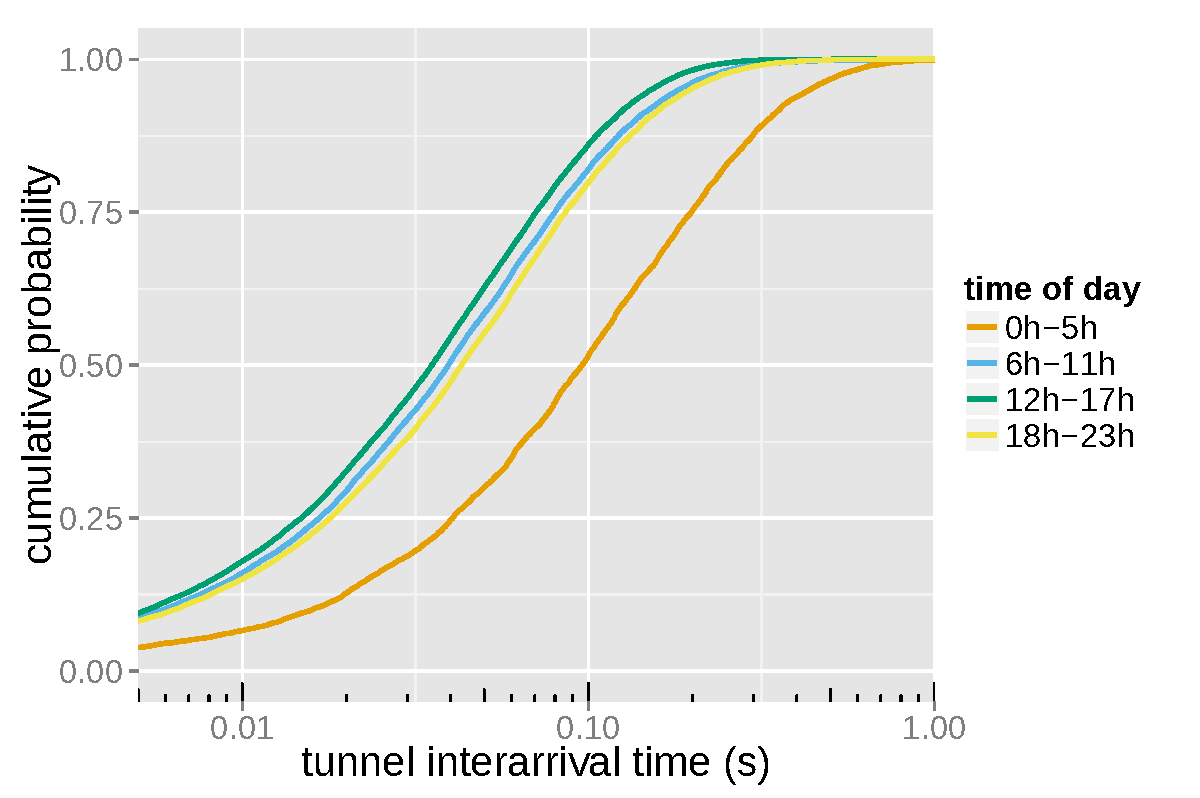
\includegraphics[width=\textwidth]{images/R-IAT-fromflows-umts-ecdfs-2h.pdf}
                \caption{Tunnels with data flows initiated in UMTS.}
                \label{c4:fig:IAT-ecdf-2h-active-umts}
        \end{subfigure}
}
        \caption{Empirical cumulative distribution function of the tunnel inter-arrival time in seconds by time of day for each day of one week.}
        \label{c4:fig:IAT-ecdf-2h}
\end{figure}

To investigate the arrivals from yet another angle we take a look at inter-arrival time of the tunnels in Figure~\ref{c4:fig:IAT-ecdf-2h}. This metric is more suited to describe the arrival process in the toy queuing model we propose. The empirical CDFs are again broken down by time of day, the same diurnal load oscillation can be observed. The medians range between about 20 and 60 milliseconds. Figure~\ref{c4:fig:IAT-ecdf-2h-all}, which represents all tunnel requests that the \gls{GGSN} received, shows wave-like steps in 20ms intervals in the plot. As this is happening very regularly at every time of the day we believe, that this effect must be from a source inside the mobile network and not induced from the outside, .e.g. through mobile devices.

This becomes even more peculiar when further breaking down the tunnel arrivals. We now distinguish between active tunnels, i.e. tunnels, that actually transported user traffic during their lifetime (cf. Fig.~\ref{c4:fig:IAT-ecdf-2h-active}), and active tunnels, which were created while having a GPRS (Fig.~\ref{c4:fig:IAT-ecdf-2h-active-gprs}) or UMTS (Fig.~\ref{c4:fig:IAT-ecdf-2h-active-umts}) connectivity, respectively. Note that only about 86\% of requested and created tunnels where actually used for user data transmissions afterwards. The 20ms-steps occur strongest when observing all tunnel arrivals, in a weaker form it is also present in the active and \gls{UMTS} tunnel portion. 

Our working hypothesis as to the origin of the effect is the \gls{TTI}. This time indicates the duration of a radio transmission and is usually either 10 or 20 milliseconds in length. It is also in sync for the whole network of base stations making the \gls{TTI} noticeable even when not measuring directly at the radio link. The observed step-width of 20ms therefore indicates, that the signaling procedure the GTP CREATE is part of, includes at least one trip from the mobile device over the radio interface. This makes sense, as the tunnel is typically created during the GPRS Attach procedure, which is indeed initiated at the user's device. Unfortunately, this also makes the tunnel arrivals come in somewhat batched, which could momentarily increase the load at the \gls{GGSN} that then would need to process more requests at once than if the arrivals followed a smooth stochastic distribution.




%%%%%%%%%%%%%%%%%%%%%%%%%%%%%%%%%%%%%%%%%%%%%%%%%%%%%%%%%%%%%%%%%%%%%%%%%%%%%%%
\subsubsection{Tunnel Event Processing Time}

This brings us to another and potentially more direct measure of \gls{GGSN} load, namely the event processing time, meaning the time it takes for the \gls{GGSN} to fulfill a \gls{GTP} request. This is calculated from the requested and finished timestamps of every \gls{GTP} event in our dataset. As the measurement is conducted at the Gn interface these timestamps represent the time the \gls{GTP} signaling request moves to the \gls{GGSN} and the time the response transitions through the link.

As stated in the previous section, it would be of special interest to know if the setup time of tunnels is influenced by anything, as this is one of the \gls{GGSN}'s most time-sensitive jobs and can impact the time a user has to wait before being able to actually transfer data. Unfortunately, some issues with the dataset did not allow the investigation of the processing time of either create and delete messages.

\begin{figure}[htbp]
	\centering
	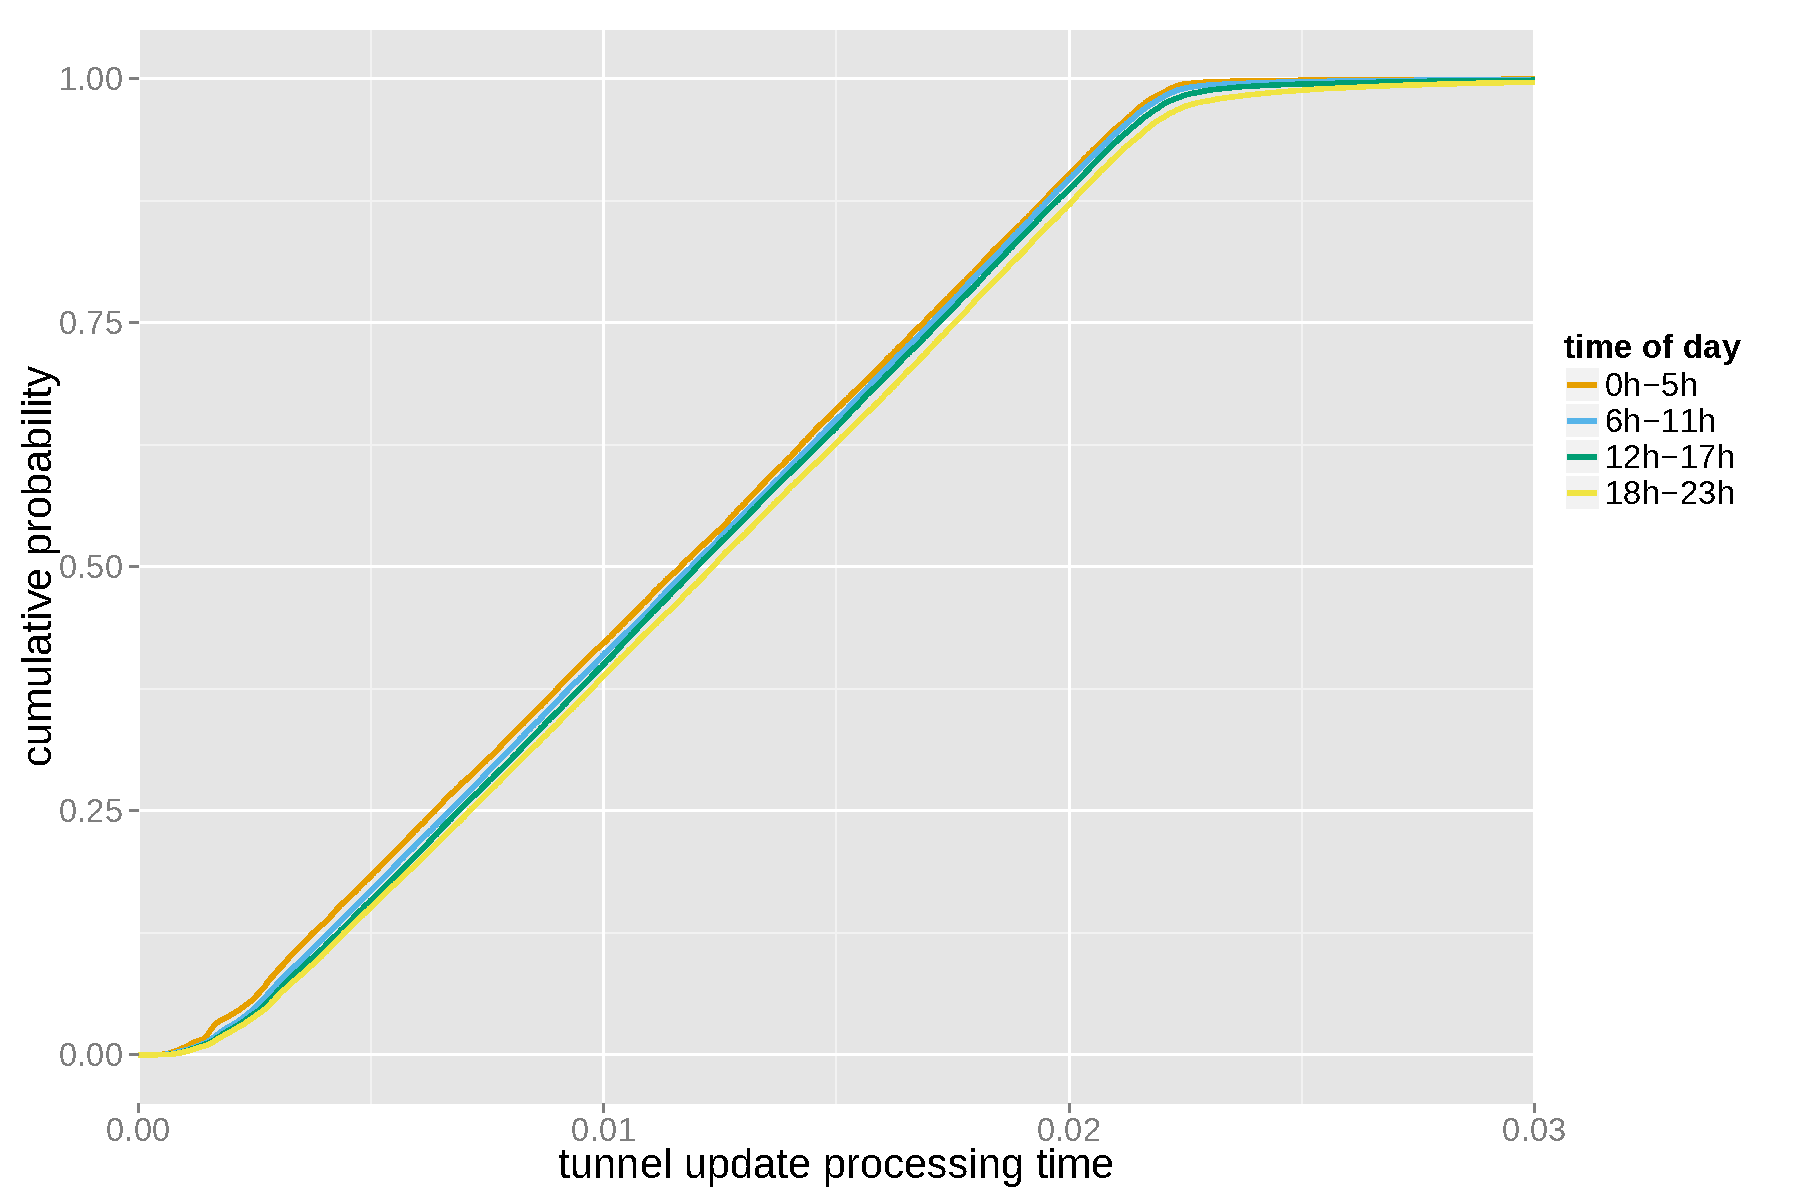
\includegraphics[width=\columnwidth]{images/R-update-time-cdfs.pdf}
	\caption{Empirical CDFs of the time it takes a GGSN to process a GTP update event, plotted for each hour of the day.}
	\label{c4:fig:update-time}
\end{figure}


However, we could investigate the processing time of \gls{GTP} update messages. The core network transmits roughly two orders of magnitude more update than either create or delete events and therefore the number of usable events exceeded the significance level. While no direct investigation of the setup and deletion procedures was possible with these events, a rough overall picture of load can still be attained through this. Figure \ref{c4:fig:update-time} depicts a band of empirical cumulative distribution functions for the processing time of update events broken down by time of day. The processing time is almost uniformly distributed between 2 and 22 milliseconds, with a slightly longer duration during the evening, making for a continuous uniform distribution. This is rather unexpected as uniform distributions do not usually occur in computing processes. According to the central limit theorem one would rather expect to see a normal distribution influenced by, e.g., scheduling or queuing artifacts. In the future we hope to investigate these features more closely, including a proper investigation of the tunnel setup and teardown processing time, if the dataset allows it.



%%%%%%%%%%%%%%%%%%%%%%%%%%%%%%%%%%%%%%%%%%%%%%%%%%%%%%%%%%%%%%%%%%%%%%%%%%%%%%%
\subsection{Statistical Evaluation and Data Fitting}
\label{c4:sec:statistical_evaluation}


\begin{figure}[htbp]
  \centering
  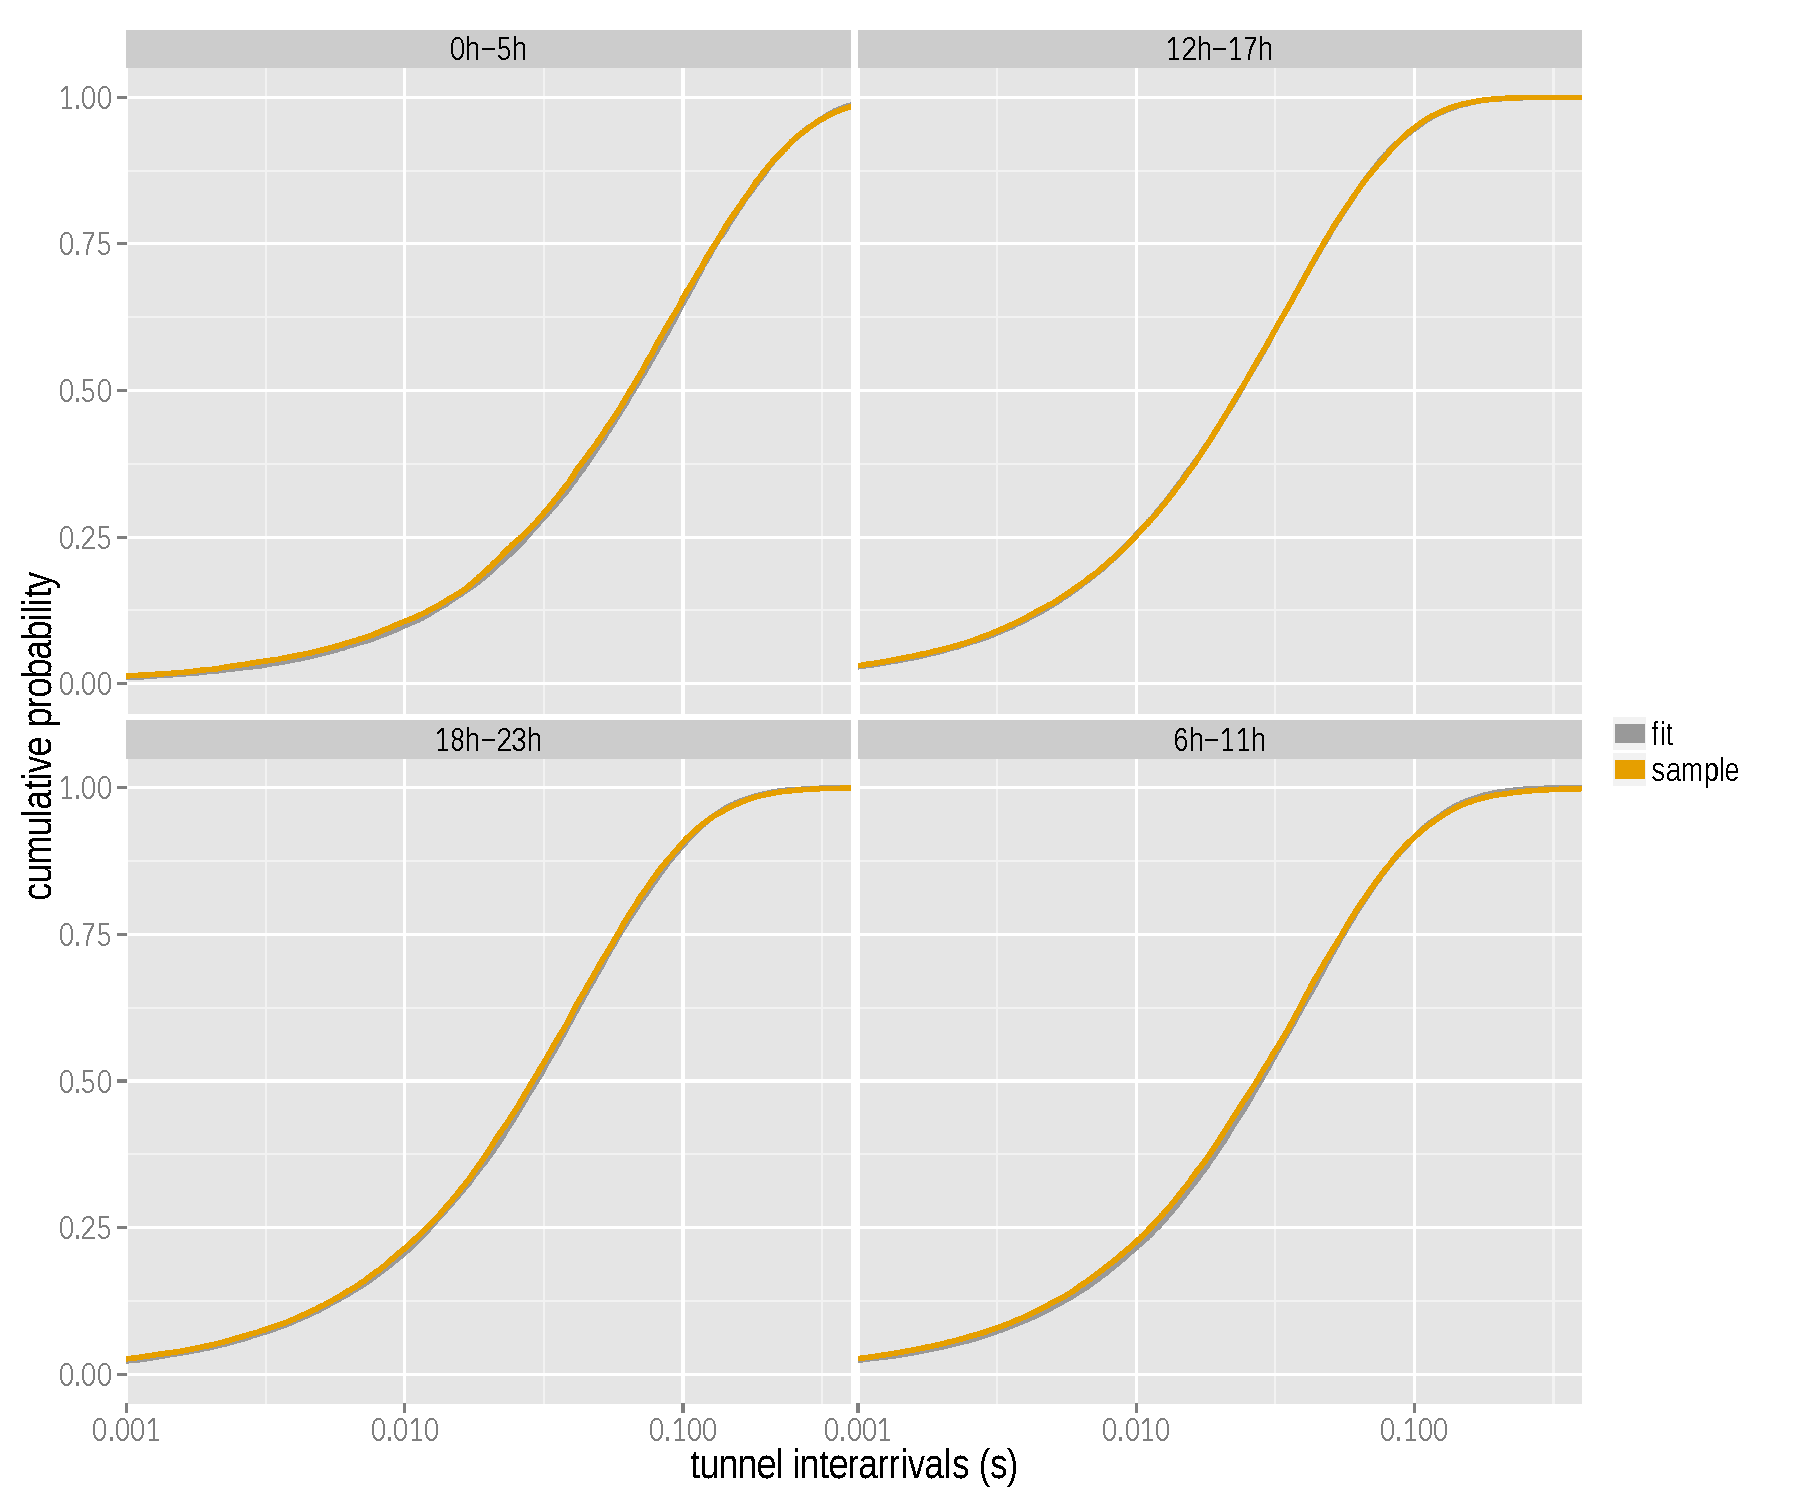
\includegraphics[width=0.8\textwidth]{images/R-IAT-active-fit-cdf-facets.pdf}
  \caption{Empirical and exponentially fitted CDFs of the tunnel interarrival duration by time of day. CDFs are overlapping as the coefficient of determination is close to $1$.}
  \label{fig:pdparrivalsecdf}
\end{figure}

Using this dataset, we can obtain the distributions required for the models. At first, we take a look at the tunnel interarrival time in Figure~\ref{fig:pdparrivalsecdf}.
%This can be a good measure for the load a \gls{GGSN} experiences, as every incoming tunnel carries several signaling interactions, processing and state with it.
Typically, a device will only hold one tunnel at a time, but this one tunnel can be initiated and shut down in rapid succession, thus causing the aforementioned issues in the radio network. The arrivals also show a strong diurnal effect, closely resembling patterns present in the actual user traffic: A decline of arrivals, i.e. longer interarrivals, late in the night and during the early morning hours with a peak rate in the afternoon and early evening. To represent this time-of-day dependence in the model, the measurement was split into the four time slots displayed in the figure. Each slot was then fitted with an exponential distribution by way of moments matching. This results in the cumulative distribution function $F(x) = 1- e^{-\lambda x}, x \geq 0$ with $\lambda$ given in Table~\ref{tab:fits} for the four time slots. The fitted functions match the empirical data quite well, with some deviation present at the left tail but overall with a positive correlation coefficient approaching 1.

\begin{figure}[htbp]
  \centering
  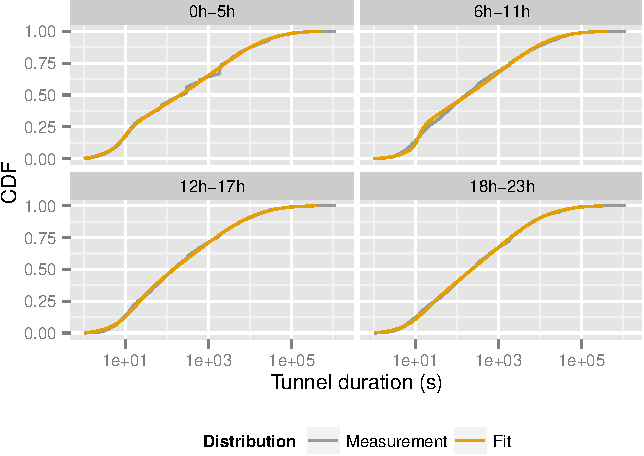
\includegraphics{images/timeslot-fits.pdf}
  \caption{Empirical and fitted CDFs of the tunnel duration by time of day with fitted rational functions.}
  \label{c4:fig:fittedsdurationlots}
\end{figure}

The second important tunnel property is the duration the \gls{PDP} Context state accompanying a \gls{GTP} tunnel is held at the \gls{GGSN}. Fig.~\ref{c4:fig:fittedsdurationlots} shows the tunnel durations split up for the time of day, as there is once again a slight diurnal effect present, albeit with shifted peaks. Longer tunnels tend to occur at night, shorter tunnels during midday.
%Further properties of the tunnel duration, especially the correlation with device types and operating systems, were already investigated in detail in our previous work \cite{metzger2012research,metzger2013}.
For the model, a distribution fit of the tunnel duration was also desired. However, none of the basic probability distributions (including exponential, gamma, and Weibull distributions) fit the tunnel duration well enough. One of the reasons for this probably being the correlation of the tunnel duration to a large number of factors, including user behavior and network-specific timers and procedures,
%Tunnels are shut down by the network after specific events (e.g. a 30-minute idle timer), 
introducing artifacts which make it hard to fit any distribution against. Instead, we fitted rational functions to the empirical CDF using Eureqa \cite{eureqa_paper, eureqa_software}. This allowed for a much closer fitting while still smoothing out some of the artifacts. Table~\ref{tab:fits} also displays these functions fitted to the inverse CDF, to be directly used for generating random numbers using the inversion method. Both the CDF in Fig.~\ref{c4:fig:fittedsdurationlots} as well as the Pearson correlation coefficient confirm the goodness of the fitted functions.


\begin{table}[htbp]
  \caption{Parameters for the exponentially distributed inter-arrival times and corresponding Pearson correlation coefficients; also contains the inverse functions fitted to the empirical duration distribution and correlation coefficients of the fit.}
  \label{tab:fits}
  \tabulinesep=1.2mm
  \centering
  \begin{tabu}{|[1.2pt]X[0.9,l]|[1.5pt]X[r]|X[r]|X[4.5,r]|X[r]|[1.5pt]} 
  %\tabucline[1pt]-
  \textbf{Time of Day} & $\mathbold{\lambda}$ & $\mathbold{R_{arrival}}$ & \textbf{Inverse Fitted Duration Function} & $\mathbold{R_{dur}}$\\ \tabucline[1pt]-\everyrow{\tabucline[on 1.5pt off 2pt] - }
  0h-5h & $10.67477$ & $0.99538$ & $0.919208 - 60.6136y - 3498.78y^3 - \frac{110.707y + 2289.94y^3}{y - 1.00469}$ &  $0.9999021$ \\
  6h-11h & $24.53298$ & $0.99216$ & $1 + 117.484y - 368.643y^2 - \frac{1720.13y^4}{y - 1.0041}$ & $0.9998909$ \\
  12h-17h & $29.2504$ & $0.99256$ & $0.952566 + 69.4907y + \frac{81146.1y^3 + 1.08572\times10^6y^5}{805 - 802.01y}$ & $0.9999027$ \\
  18h-23h & $23.49983$ & $0.98617$ & $0.911924 + 82.0562y - \frac{2936.93y^4}{1.94468y - 1.9532}$ & $0.9998071$  %\everyrow{} \\ \tabucline[1.2pt]-
  \end{tabu}
\end{table}




%% to be integrated into evaluation
\begin{figure}[htbp]
  \centering
  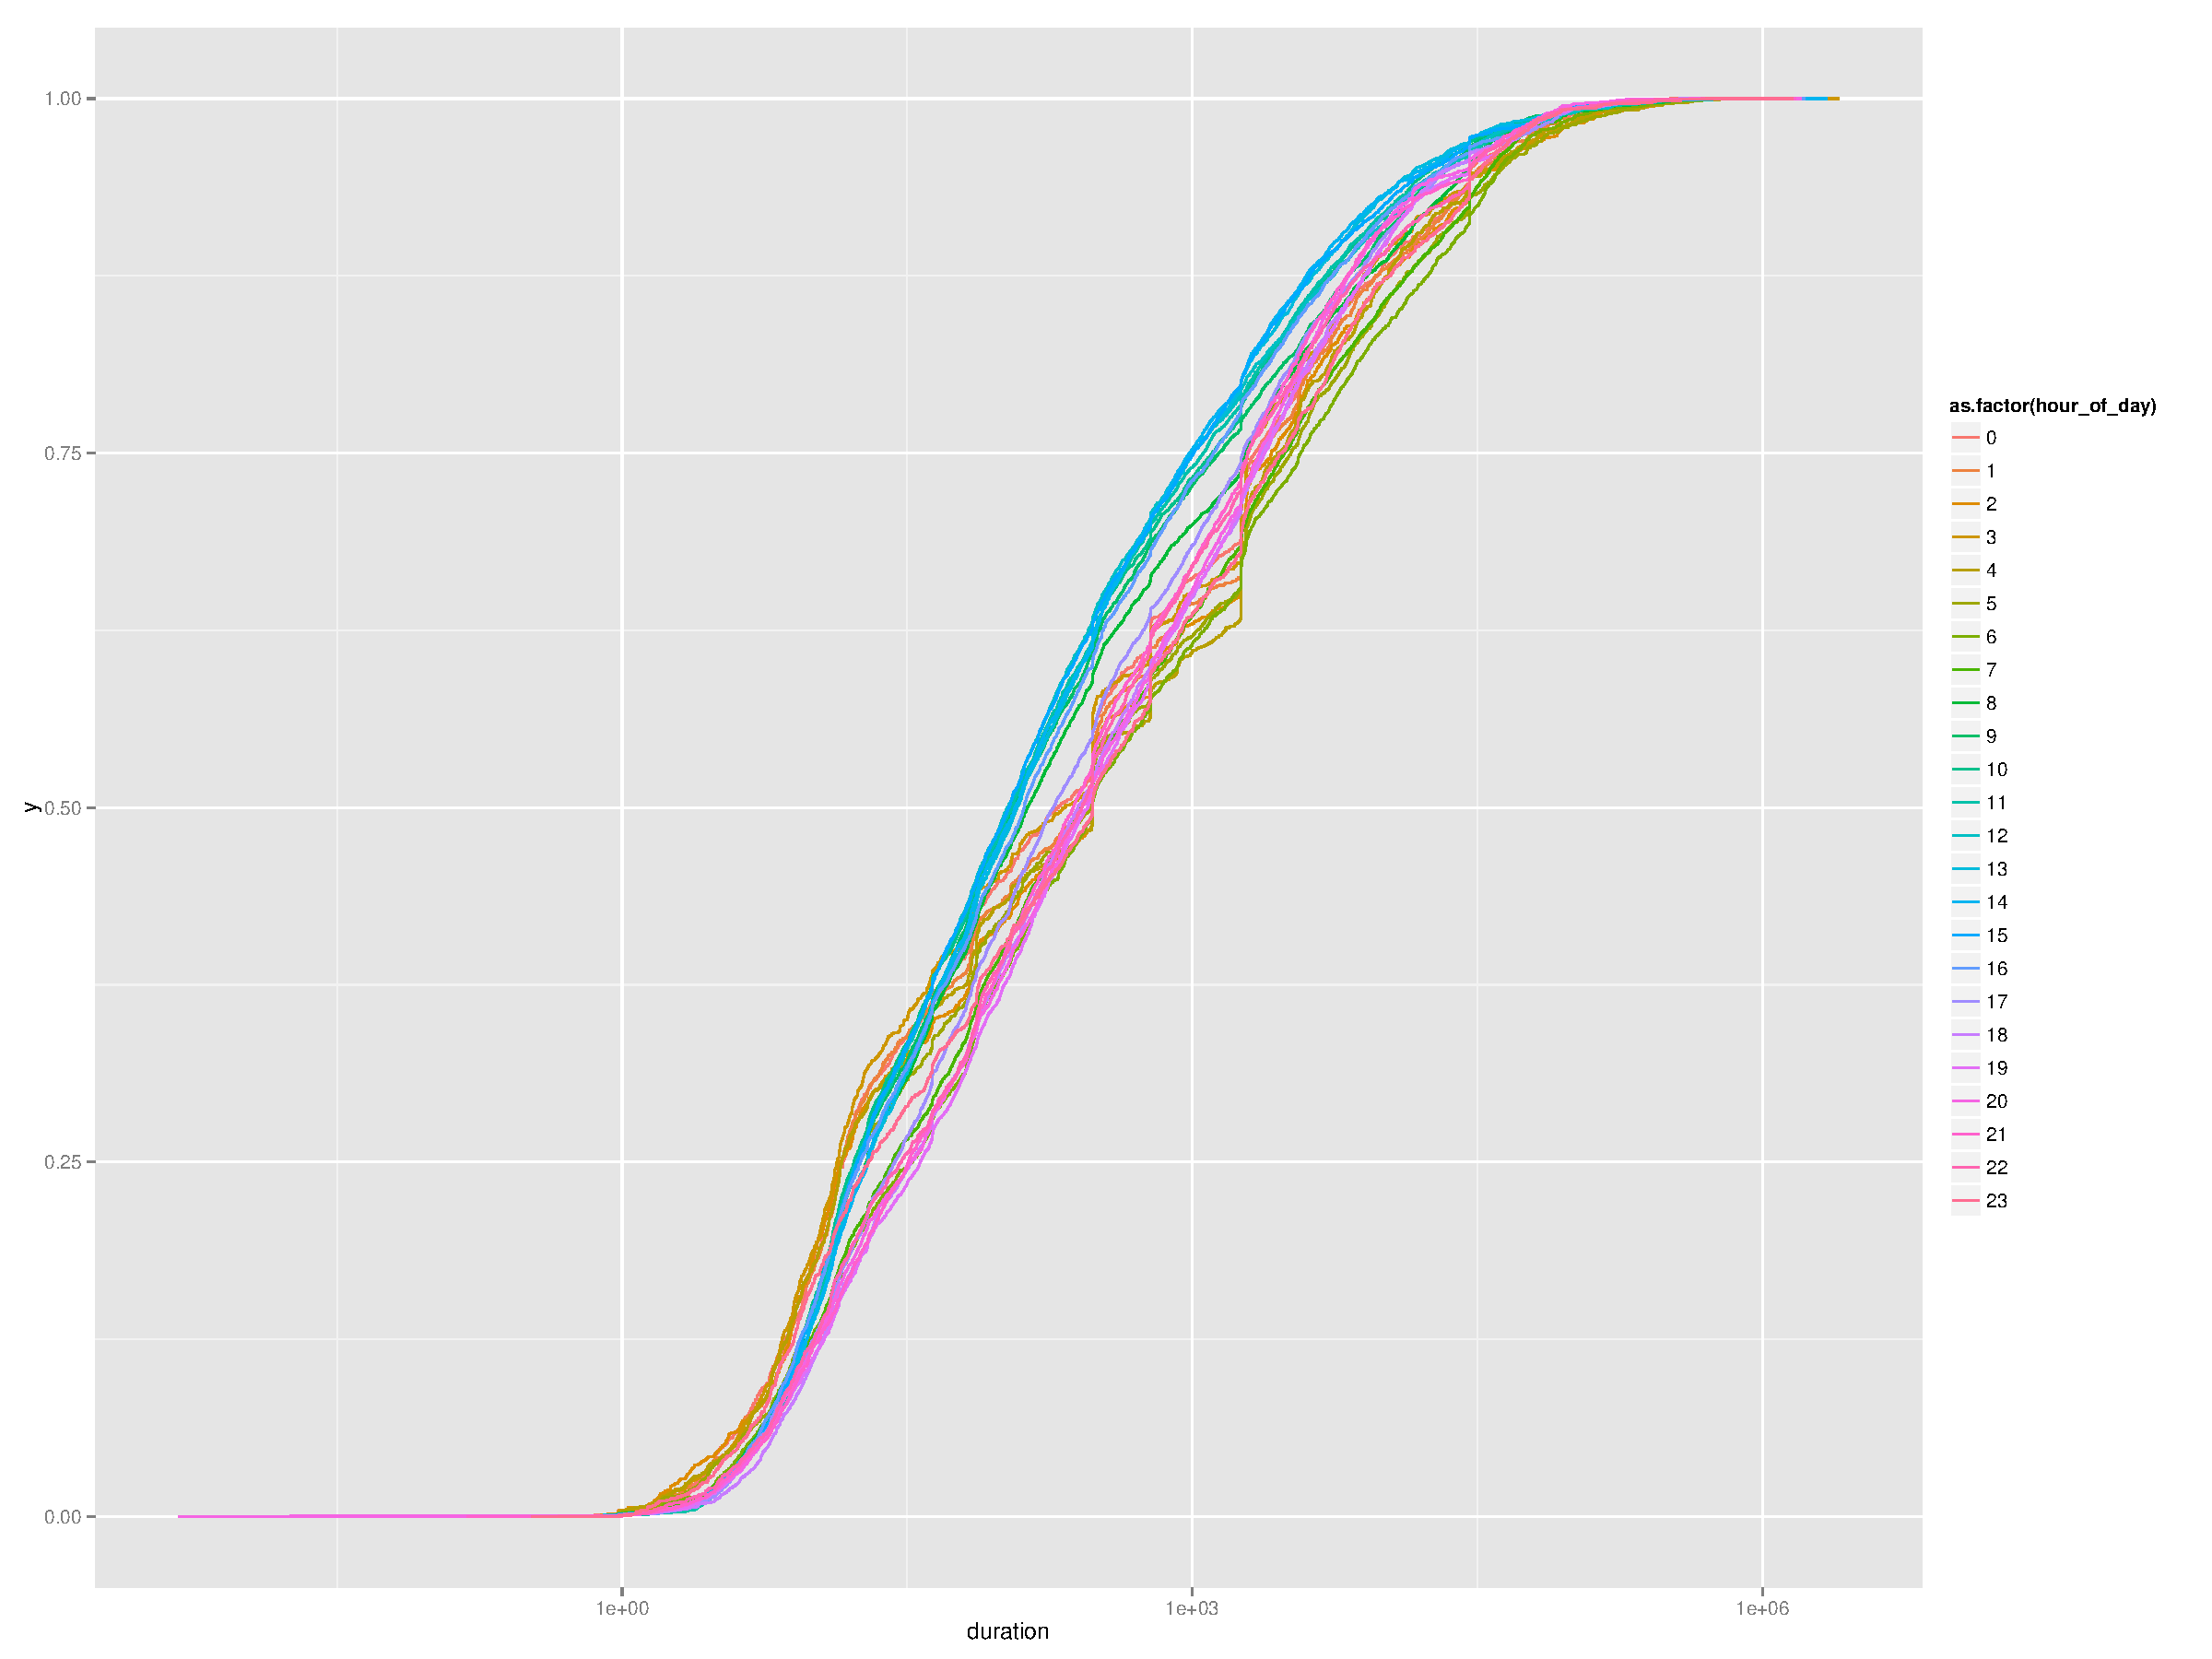
\includegraphics[width=1.0\textwidth]{images/R-duration-activetunnels-hours-ecdf.pdf}
  \caption{Tunnel duration of all active tunnels by time of day.}
 \label{c4:fig:duration-timeofday-ecdf}
\end{figure}